%% An Introduction to LaTeX Thesis Template of Wuhan University
%%
%% Created by WHUTUG

\documentclass[type=bachelor]{whu-thesis}
\whusetup
  {
    info               =
      {
         title          = {基于统计的基本面分析},
        title*         = {An Introduction to LaTeX Thesis Template\\of Wuhan University},
        student-number = {2017302010265},
        school         = {经济与管理学院},
        author         = {鲍余薇},
        author*        = {Yuwei Bao},
        subject        = {学科},
        major          = {金融工程},
        advisor        = {李斌 , 教授},
        direction      = {研究方向},
        % date           = {2021/2},
        keywords       = {关键词 1 , 关键词 2 , 关键词 3 , 关键词 4 , 一个非常非常,非常非常长——的关键词 5},
        keywords*      = {key word 1 , key word 2 , key word 3 , key word 4 , {and a very very, very very long key word---the key word 5}},
      },
    style              =
      {
        graphics-path  = {{figures/}{data/}},
        list-of-figures,
        list-of-tables,
      },
    element            =
      {
        innovation     = {pages/innovation},
        abstract       = {pages/abstract},
        abstract*      = {pages/enabstract},
        bibliography   = {ref/zotero},
        achievements   = {pages/achievements},
        thanks         = {pages/thanks},
        %appendix       = {pages/appendix}
      }
  }

\begin{document}
%%----------- 主体部分 ----------- %%
% Chapter1

\chapter{引言}
有效市场假说(Efficient Markets Hypothesis,EMH)是现代金融学的理论基石之一。Fama(1965)首次提出了“有效市场”的概念,并定义为:如果在一个证券市场中,价格完全反映了所有可以获得的讯息,那么就称这样的市场为有效市场。他认为市场上存在着大量理性的投资者,在任何时间都有无数人正在搜寻细微的线索去精准预测股票未来的价格,为了自身利益去对股票进行低买高卖,或许对于个人而言仅仅是超额利润的攫取,但在宏观维度上,正是这种高量级的活动快速推进着股票市场价格向正确价格的趋近,任何相关的信息已经完全展现在了股票价格中,所有为了预测付出的时间、金钱和努力都是徒劳无功。进而Fama(1970)在《Journal of Finance》杂志上发表了最具划时代意义的论文《Efficient Capital Markets: A Review of Theory and Empirical Work》,正式提出了有效市场假说,并对证券市场的信息分为以下三类:一是与交易相关的历史信息,例如历史成交量、价格等;二是当前的公开信息,如公司财报、分红报告等;三是内部信息。Fama按照以上三种信息把有效市场分为弱式有效、半强式有效和强式有效三类,其中弱式有效证明了技术分析的无效性;半强式有效排除了基本面分析的作用;而强式有效意味着股票价格已经反映了所有信息,投资者不可能战胜市场。至此确立了“有效市场假说”在现代金融领域的基础性地位。

但是现在越来越多的实证研究表明了中国股票市场的非有效性。自70年代开始,随着科技的发展,持续识别出能够提供超额收益的异象(因子)。曾有研究发现了股票价格过度波动和可预测性(Shiller,1981)、股票价格走势逆转(Shieifer、Vishney,1994)等异常情况;在单只股票或投资组合领域,也发现了规模效应(Bamber等,1997)、市盈率效应(Banz,1981)等,前美国金融学会主席Cochrane(2011)称其为“因子动物园”(Factor Zoo),这些异象说明投资者能够基于基本面等公开信息去预测股票价格,向有效市场假说发起了挑战。

另外,从行为金融角度看,很多学者指出有效市场假说理论的逻辑存在问题。如果股票价格已经完全反映市场中的信息,那理性投资者在后续的投资活动中就无需花费精力去搜集信息、预测股价了,但这却与市场需要信息才能有效运行相悖。同样,其设定的完美市场假定条件脱离实际。在实际的投资活动中,投资者更多表现为“非理性”,从而导致其决策行为偏离金融理论预测的标准结果,例如羊群效应、月末效应、规模效应和股权溢价之谜等等金融异象都是投资者“非理性”行为的表现(张元鹏,2015)。虽然行为金融文献并没有完全否定有效市场的界定,但行为金融派的支持者更愿将有效市场看作一种理想状态、不受个人意志(效用和偏好)影响的市场状态(丁志国等,2017)。

从以上几个方面来看,我国股票市场未能做到完全有效,虽然A股市场现已发展成为全球第二大股票市场,总市值近80万亿元。但由于成立时间晚、相关制度不完善、散户比例大、交易成本高等问题,导致了定价效率的低下。这时基本面分析更能捕捉市场的非有效性,有效预测未来盈余,带来显著的超额回报(汪荣飞和张然,2018)。相对于技术分析依靠图表去预测价格趋势,基本面分析更为关注公司的基本信息,主要包括财务报表或非财务上的信息,并从中评估公司的内在价值。本文将股票价格与内在价格的偏离定义为错误定价,而这种错误定价便是投资者所追捧的超额收益,所以对于错误定价的研究显得极为重要。

由于股票价格是已知的,那么对错误定价的研究关键在于对股票内在价格、公司内在价值的预测。现有研究中常见的计算方法包括现金流贴现法(Free Cash Flow Valuation,FCFF);相对价值法,即与同行业的相似公司对比,以它们的平均市盈率、市净率及市销率等指标来计算;经济附加值法(Economic Value Added,EVA);实物期权法等。这些方法虽然起到了一定的预测作用,但由于其选择的指标过少,或太过于依赖对未来的主观预测结果,亦或计算方法过于程式化等原因,很难排除数据窥视(Data snooping)的影响。

基于以上分析,本文创新采用大数据统计方法计算公司的内在价值。利用2003年初到2020年底的季度财务报表数据,对A股所有公司(剔除金融类股票、ST股票)进行时间维度的截面回归:公司市场价值对于一系列财务指标的线性回归,这些财务指标的组合结果即为公司内在价值,回归残差为公司市场价值与内在价值的偏差,将偏差按照公司市场价值标准化后,成功构建出错误定价因子M(Mispricing Factor)。其中,线性回归系数按时点分组截面计算,避免了该时点下其他投资因素的影响;纳入A股所有公司,回归结果更具有普遍性;且后续模型修订根据客观统计标准,排除了数据窥视的影响。

在成功引入错误定价因子M后,接下来便是检验其有效性。问题在于:一、能否通过错误定价因子M构建低买高卖的投资组合获取超额收益,进而证明基本面分析的可行性?二、超额利润来自于错误定价还是因子遗漏,股票市场价格是否会向内在价格趋近?本文将针对以上两个问题进行研究。首先从CSMAR上搜集A股上市公司季度财务数据,计算每个时点公司的内在价值和错误定价因子M;后采用Fama-MacBeth回归计算错误定价因子M系数$\beta$,检验其是否显著;并且按照错误定价因子M将公司分为五组,从价值最被高估到最被低估,运用因子模型得超额收益$\alpha$,观察是否呈现单增趋势;最后观察长期时间内不同分组超额收益的变动趋势,证明超额收益并非来源于风险因子的遗漏。最后结论证明了错误定价因子M的有效性,有力支持了基本面分析之于中国股市证券分析的地位。

本文的研究有一定的现实意义与理论贡献:一、丰富了经济学和管理学研究的工具箱;二、丰富了基本面投资的理论和实践研究;三、丰富了中国股票市场有效性的研究。目前对于中国A股市场基本面分析的研究过少且不完善,以大数据统计方法的研究更为稀有,统计之于数据分析的重要性不言而喻,其能够有效避免数据窥视的影响,是在此研究方向上的创新。同样,建模方法也有所创新,在线性回归的基础上增加了非线性维度的考量。

后文结构如下:第二部分回顾了中国股市有效性、基本面分析等相关文献,第三部分阐述了本文的研究设计,介绍数据和变量的构建方法;第四部分详细分析了本文的实证结果,第五部分为本文的研究结论。

% Chapter 2

\chapter{文献综述}
对于中国股票市场,已有多位学者研究证明其不具有弱势有效性。
\citeauthor{jiaZhongGuoGuShiYouXiaoXingDeShiZhengFenXi2003}(\citeyear{jiaZhongGuoGuShiYouXiaoXingDeShiZhengFenXi2003})对基于市场有效假设的CAPM模型以及其他因素与收益率之间的关系进行了实证检验,发现目前我国股市不满足市场有效性的假设,投资者的行为并不是完全理性的;
\citeauthor{wuZhongGuoGuPiaoShiChangRuoYouXiaoXingDeTongJiTaoLiJianYan2007}(\citeyear{wuZhongGuoGuPiaoShiChangRuoYouXiaoXingDeTongJiTaoLiJianYan2007})通过设计多种投资组合方式,发现在短期(3个月以内)不能否定市场中无套利的假定;而对于中期和长期(6个月及12个月) 统计套利存在,说明我国A股股票市场的弱有效性不成立;
\citeauthor{limAreChineseStock2009}(\citeyear{limAreChineseStock2009})运用非线性依赖检验的方法对1999年至2005年上证A股和B股的日数据进行检验,发现A股和B股均不具备弱势有效性;
\citeauthor{quJiYuXuLieXingZhiJianYanDeZhongGuoGuPiaoShiChangRuoShiYouXiaoXingYanJiu2014}(\citeyear{quJiYuXuLieXingZhiJianYanDeZhongGuoGuPiaoShiChangRuoShiYouXiaoXingYanJiu2014})利用Q统计量法、方差比检验法、广义谱检验、游程检验等多种方法对2010年至2013年沪深300股指期货的当月合约的5分钟高频数据进行检验,实证结果表明,随着考察期长度的增加,市场趋于拒绝弱式有效性。

上述研究说明,中国股市能够通过技术分析和基本面分析获取超额收益,实际上很
多实证研究也证明了这个结论。
对于技术分析,\citeauthor{zhaoJiYuShiJianXuLieFenXiDeGuPiaoJieGeQuShiYuCeYanJiu2009}(\citeyear{zhaoJiYuShiJianXuLieFenXiDeGuPiaoJieGeQuShiYuCeYanJiu2009})基于时间序列方法,使用GARCH模型和ARIMA模型对股价波动趋势有着较好的短期预测效果;
\citeauthor{wangGuShiChangYongJiShuFenXiFangFaDeYouXiaoXingShiZhengYanJiu2010}(\citeyear{wangGuShiChangYongJiShuFenXiFangFaDeYouXiaoXingShiZhengYanJiu2010})运用技术指标MA、KDJ和MACD证明在一定时间跨度上技术分析是有效的;
\citeauthor{shiGuPiaoJiShuFenXiZhongMACDZhiBiaoDeYouXiaoXingJianYan2011}(\citeyear{shiGuPiaoJiShuFenXiZhongMACDZhiBiaoDeYouXiaoXingJianYan2011})的实证研究表明MACD指标对于2004年至2009年内的大、中、小盘股均有一定的预测能力;
\citeauthor{baoZhongGuoGuShiJiShuFenXiYouXiaoXingYanJiu2015}(\citeyear{baoZhongGuoGuShiJiShuFenXiYouXiaoXingYanJiu2015})基于2010到2014年三只指数标的和一只个股标的,通过持续持有策略和均线穿越法则策略获取了超额收益。

对于基本面分析,\citeauthor{zhangFenXiShiXiuZhengXinXiJiBenMianFenXiYuWeiLaiGuPiaoShouYi2017}(\citeyear{zhangFenXiShiXiuZhengXinXiJiBenMianFenXiYuWeiLaiGuPiaoShouYi2017})采用日历时间组合的方法,证实中国A股市场的分析师修正信息具有投资价值,并且这个投资价值主要来源于其能够预测公司基本面信息。
\citeauthor{wangJiBenMianFenXiZaiZhongGuoAGuShiChangYouYongMaLaiZiJiDuCaiWuBaoBiaoDeZhengJu2018}(\citeyear{wangJiBenMianFenXiZaiZhongGuoAGuShiChangYouYongMaLaiZiJiDuCaiWuBaoBiaoDeZhengJu2018})基于季度财务指标构建了六组基本面指标,发现均能够有效预测未来盈余,进而发现分析师和投资者均没有意识到基本面指标的价值。
\citeauthor{changJieZhiYinZiBeiHouDeLuoJiGuZhiJiBenMianYuQiChaiYuCuoWuDingJie2020}(\citeyear{changJieZhiYinZiBeiHouDeLuoJiGuZhiJiBenMianYuQiChaiYuCuoWuDingJie2020})构建了价值因子、基本面两个维度进行横截面分析,发现只有当估值和基本面预期背离、存在错误定价时,高低估值的对冲组合才能产生显著的超额收益,高达16.8\%。

目前国内有关基本面分析的研究较少,但在成熟的国外资本市场,基本面分析的作用已被大量文献证实。
\citeauthor{ouInancialStatementAnalys1988}(\citeyear{ouInancialStatementAnalys1988})构建了68组基本面指标,发现其能够成功预测未来股票收益涨跌的概率,多空组合在两年内达到12.5\%的超额收益。
\citeauthor{abarbanellFundamentalAnalysisFuture21}(\citeyear{abarbanellFundamentalAnalysisFuture21})构建了12组基本面指标,研究发现大部分指标能够预测股票未来价值,
\citeauthor{abarbanellAbnormalReturnsFundamental1998}(\citeyear{abarbanellAbnormalReturnsFundamental1998})进一步利用这些基本面指标构建投资组合,获得了13.2\%的年化超额收益,并发现超额收益大部分与未来的业绩公告相关。
\citeauthor{piotroskiValueInvestingUse2000}(\citeyear{piotroskiValueInvestingUse2000})对高账面市值比的公司进行了研究,并用9组基本面指标构建出综合指标FSCORE,用FSCORE挑选出真正的价值股并提升了7.5\%的收益率。
同样,\citeauthor{mohanramSeparatingWinnersLosers}(\citeyear{mohanramSeparatingWinnersLosers})着眼于低账面市值比的成长股,利用8组基本面指标构建了综合指标GSCORE。
\citeauthor{asnessQualityMinusJunk2019}(\citeyear{asnessQualityMinusJunk2019})根据盈利性、成长性、安全性,构建了衡量公司质量的QMJ(quality minus junk)指标,发现高质量公司股价较高,但低质量公司不定,多头高质量公司空头低质量公司的投资组合信息比率大于1。
\citeauthor{bartramAgnosticFundamentalAnalysis2018a}(\citeyear{bartramAgnosticFundamentalAnalysis2018a})基于统计方法对在CRSP有记录的美国公司进行连续310月的检验,发现错误定价信号能够预测未来收益,带来超额利润,基本面分析有效。

上述研究均根据基本面指标构建了综合指标,并且构建对应的多空组合获取了超额收益,证明了基本面分析的有效性。但国内有关基本面分析的研究较少,运用大数据统计方法、机器学习算法的更少。
\citeauthor{liMLTEAYiTaoJiYuJiQiXueXiHeJiShuFenXiDeLiangHuaTouZiSuanFa2017}(\citeyear{liMLTEAYiTaoJiYuJiQiXueXiHeJiShuFenXiDeLiangHuaTouZiSuanFa2017})设计了一套基于机器学习和技术指标的量化投资算法ML-TEA(Machine Learning and Technical Analysis),分别采用支持向量机、神经网络、Adaboost 等机器学习算法,利用19项技术指标预测股价涨跌方向,发现这些算法具有更高的预测准确率, 而根据预测所构建的投资组合也取得了更好的投资绩效。
进而\citeauthor{liJiQiXueXiQuDongDeJiBenMianLiangHuaTouZiYanJiu2019}(\citeyear{liJiQiXueXiQuDongDeJiBenMianLiangHuaTouZiYanJiu2019})基于A股市场的96项异象因子,运用12种机器学习算法去构建股票收益预测模型及投资组合,并且其投资策略能够获得比传统线性算法和所有单因子更好的投资绩效。
\citeauthor{fischerDeepLearningLong2018}(\citeyear{fischerDeepLearningLong2018})采用长短期记忆模型(Long Short-Term Memory,LSTM),利用日频收益率数据预测标普500中的每只成分股相对于其截面中值收益率的涨跌方向, 而相应构建的投资组合绩效显著优于其他线性或机器学习模型。

综上所述,本文将通过BRTs模型,基于A股公司财务指标去进行其内在价值的预测,并以内在价值与市场价值的差异去构建错误定价因子$M$,以此进行我国A股市场基本面分析可行性的研究。


%\section{公式的使用}
%在文中引用公式可以这么写:\(a^2 + b^2 = c^2\)。这是勾股定理,它还可以表示为 \(c = \sqrt{a^2 + b^2}\)。还可以让公式单独一段并且加上编号:
%注意,公式前请不要空行。
%
%还可以通过添加标签在正文中引用公式,如式\eqref{eq:pingfanghe}。
%
%我们还可以轻松打出一个漂亮的矩阵:
%\begin{equation}
%  \vb*{A} =
%  \begin{bmatrix}
%    1  & 2  & 3  & 4  \\
%    11 & 22 & 33 & 44 \\
%  \end{bmatrix} \times
%  \begin{bmatrix}
%    22 & 24 \\
%    32 & 34 \\
%    42 & 44 \\
%    52 & 54 \\
%  \end{bmatrix}
%\end{equation}
%
%或者多行对齐的公式:
%\begin{equation}
%  \begin{aligned}
%    f_1(x) & = (x + y)^2         \\
%           & = x^2 + 2 x y + y^2
%  \end{aligned}
%\end{equation}
%
%模板使用了 unicode-math 包更改数学字体。所以在使用数学字体时,尽量使用 unicode-math 包提供的 \verb|\sym| 接口,详情请阅读 unicode-math 文档。
%
%\section{插图的使用}
%\begin{figure}
%  \centering
%  \includegraphics[width=0.3\textwidth]{whulogo.pdf}
%  \caption{插图示例}
%  \label{fig:whu}
%\end{figure}
%
%\LaTeX{} 环境下可以使用常见的图片格式:JPEG、PNG、PDF 等。当然也可以使用 \LaTeX{} 直接绘制矢量图形,可以参考 pgf/ti\emph{k}z 等包中的相关内容。需要注意的是,无论采用什么方式绘制图形,首先考虑的是图片的清晰程度以及图片的可理解性,过于不清晰的图片将可能会浪费很多时间。
%
%\verb|[htbp]| 选项分别是此处、页顶、页底、独立一页。\verb|[width=\textwidth]| 让图片占满整行,或 \verb|[width=2cm]| 直接设置宽度。可以随时在文中进行引用,如图~\ref{fig:whu},建议缩放时保持图像的宽高比不变。
%
%如果一个图由两个或两个以上分图组成时,各分图分别以(a)、(b)、(c)...... 作为图序,并须有分图题。模板使用 subcaption 宏包来处理,比如图~\ref{fig:subfig-a} 和图~\ref{fig:subfig-b}。
%
%\begin{figure}[h]
%  \centering
%  \begin{subfigure}{0.2\textwidth}
%    \includegraphics[width=\linewidth]{whulogo.pdf}
%    \caption{武汉大学校徽}
%    \label{fig:subfig-a}
%  \end{subfigure}\qquad
%  \begin{subfigure}{0.7\textwidth}
%    \includegraphics[width=\linewidth]{whu.pdf}
%    \caption{武汉大学}
%    \label{fig:subfig-b}
%  \end{subfigure}
%  \caption{多个分图的示例}
%  \label{fig:multi-image}
%\end{figure}
%
%\section{表格的使用}
%表格的输入可能会比较麻烦,可以使用在线的工具,如 \href{https://www.tablesgenerator.com/}{Tables Generator} 能便捷地创建表格,也可以使用离线的工具,如 \href{https://ctan.org/pkg/excel2latex}{Excel2LaTeX} 支持从 Excel 表格转换成 \LaTeX{} 表格。\href{https://en.wikibooks.org/wiki/LaTeX/Tables}{LaTeX/Tables} 上及 \href{https://www.tug.org/pracjourn/2007-1/mori/mori.pdf}{Tables in LaTeX} 也有更多的示例能够参考。
%
%\subsection{普通表格}
%下面是一些普通表格的示例:
%
%\begin{table}[ht]
%  \centering
%  \caption{简单表格}
%  \label{tab:1}
%  \begin{tabular}{|l|c|r|}
%    \hline
%    我是 & 一只 & 普通 \\
%    \hline
%    的   & 表格 & 呀   \\
%    \hline
%  \end{tabular}
%\end{table}
%
%也可以使用 booktabs 包创建三线表。
%
%\begin{table}[ht]
%  \centering
%  \caption{一般三线表}
%  \label{tab:2}
%  \begin{tabular}{ccc}
%    \toprule
%    姓名 & 学号 & 性别 \\
%    \midrule
%    张三 & 001  & 男   \\
%    李四 & 002  & 女   \\
%    \bottomrule
%  \end{tabular}
%\end{table}
%
%三线表中三条横线分别使用 \verb|\toprule|、\verb|\midrule| 与 \verb|\bottomrule|。若要添加 \(m\)--\(n\) 列的横线,可使用 \verb|\cmidrule{m-n}| 。
%
%要创建占满给定宽度的表格需要使用到 tabularx 包提供的 tabularx 环境。引用表格与其它引用一样,只需要如表~\ref{tab:3}。
%
%\begin{table}[ht]
%  \centering
%  \caption{占满文字宽度的三线表}
%  \label{tab:3}
%  \begin{tabularx}{\textwidth}{CCCC}
%    \toprule
%    序号 & 年龄 & 身高   & 体重  \\
%    \midrule
%    1    & 14   & 156    & 42    \\
%    2    & 16   & 158    & 45    \\
%    3    & 14   & 162    & 48    \\
%    4    & 15   & 163    & 50    \\
%    \cmidrule{2-4} %添加2-4列的中线
%    平均 & 15   & 159.75 & 46.25 \\
%    \bottomrule
%  \end{tabularx}
%\end{table}
%
%\subsection{跨页表格}
%跨页表格常用于附录(把正文懒得放下的实验数据统统放在附录的表中)。一般使用 longtable 包提供的 longtable 环境。若要要创建占满给定宽度的跨页表格,可以使用 xltabular 包提供的 xltabular 环境,使用方法与 longtable 类似。以下是一个文字宽度的跨页表格的示例:
%
%\begin{xltabular}{\textwidth}{CCCCCCCCC}
%  \caption{文字宽度的跨页表格示例}  \\
%  \toprule
%  1 & 0 & 5 & 1 & 2 & 3 & 4 & 5 & 6 \\
%  \midrule
%  \endfirsthead
%
%  \multicolumn{9}{l}{接上一页}      \\
%  \toprule
%  1 & 0 & 5 & 1 & 2 & 3 & 4 & 5 & 6 \\
%  \midrule
%  \endhead
%
%  \toprule
%  \multicolumn{9}{r}{转下一页}
%  \endfoot
%
%  \bottomrule
%  \endlastfoot
%
%  1 & 0 & 5 & 1 & 2 & 3 & 4 & 5 & 6 \\
%  1 & 0 & 5 & 1 & 2 & 3 & 4 & 5 & 6 \\
%  1 & 0 & 5 & 1 & 2 & 3 & 4 & 5 & 6 \\
%  1 & 0 & 5 & 1 & 2 & 3 & 4 & 5 & 6 \\
%  1 & 0 & 5 & 1 & 2 & 3 & 4 & 5 & 6 \\
%  1 & 0 & 5 & 1 & 2 & 3 & 4 & 5 & 6 \\
%  1 & 0 & 5 & 1 & 2 & 3 & 4 & 5 & 6 \\
%  1 & 0 & 5 & 1 & 2 & 3 & 4 & 5 & 6 \\
%  1 & 0 & 5 & 1 & 2 & 3 & 4 & 5 & 6 \\
%  1 & 0 & 5 & 1 & 2 & 3 & 4 & 5 & 6 \\
%  1 & 0 & 5 & 1 & 2 & 3 & 4 & 5 & 6 \\
%  1 & 0 & 5 & 1 & 2 & 3 & 4 & 5 & 6 \\
%  1 & 0 & 5 & 1 & 2 & 3 & 4 & 5 & 6 \\
%  1 & 0 & 5 & 1 & 2 & 3 & 4 & 5 & 6 \\
%  1 & 0 & 5 & 1 & 2 & 3 & 4 & 5 & 6 \\
%  1 & 0 & 5 & 1 & 2 & 3 & 4 & 5 & 6 \\
%  1 & 0 & 5 & 1 & 2 & 3 & 4 & 5 & 6 \\
%  1 & 0 & 5 & 1 & 2 & 3 & 4 & 5 & 6 \\
%  1 & 0 & 5 & 1 & 2 & 3 & 4 & 5 & 6 \\
%  1 & 0 & 5 & 1 & 2 & 3 & 4 & 5 & 6 \\
%\end{xltabular}
%
%
%\section{列表的使用}
%下面演示了创建有序及无序列表,如需其它样式,\href{https://www.latex-tutorial.com/tutorials/lists/}{LaTeX Lists} 上有更多的示例。
%
%\subsection{有序列表}
%这是一个计数的列表
%\begin{enumerate}
%  \item 第一项
%        \begin{enumerate}
%          \item 第一项中的第一项
%          \item 第一项中的第二项
%        \end{enumerate}
%  \item 第二项
%        \begin{enumerate}[label=(\roman*)]
%          \item 第一项中的第一项
%          \item 第一项中的第二项
%        \end{enumerate}
%  \item 第三项
%\end{enumerate}
%
%\subsection{不计数列表}
%这是一个不计数的列表
%\begin{itemize}
%  \item 第一项
%        \begin{itemize}
%          \item 第一项中的第一项
%          \item 第一项中的第二项
%        \end{itemize}
%  \item 第二项
%  \item 第三项
%\end{itemize}
%
%\begin{table}[b]
%  \caption{模板定义的数学环境}\label{tab:数学环境}
%  \begin{tabularx}{\textwidth}{CCCC}
%    \toprule
%    theorem     & definition & lemma  & corollary \\
%    定理        & 定义       & 引理   & 推论      \\
%    \midrule
%    proposition & example    & remark & proof     \\
%    性质        & 例         & 注     & 证明      \\
%    \bottomrule
%  \end{tabularx}
%\end{table}
%
%\section{数学环境的使用}
%模板简单定义了 8 种数学环境,具体见表~\ref{tab:数学环境},使用方法如下所示。
%
%\begin{theorem}
%  设向量 \(\vb*{a} \neq \vb*{0}\),那么向量 \(\vb*{b} \parallel \vb*{a}\) 的充分必要条件是:存在唯一的实数 \(\lambda\),使 \(\vb*{b} = \lambda \vb*{a}\)。
%\end{theorem}
%\begin{definition}
%  这是一条定义。
%\end{definition}
%\begin{lemma}
%  这是一条引理。
%\end{lemma}
%\begin{corollary}
%  对数轴上任意一点 \(P\),轴上有向线段 \(\overrightarrow{OP}\) 都可唯一地表示为点 \(P\) 的坐标与轴上单位向量 \(\vb*{e}_u\) 的乘积:\(\overrightarrow{OP} = u \vb*{e}_u\)。
%\end{corollary}
%\begin{proposition}
%  这是一条性质。
%\end{proposition}
%\begin{example}
%  这是一条例。
%\end{example}
%\begin{remark}
%  这是一条注。
%\end{remark}
%\begin{proof}
%  留作练习。
%\end{proof}
%
%若要定义自己的数学环境,可通过如下代码实现:
%\begin{verbatim}
%\newtheorem{nonsense}{胡说}
%\newtheorem*{bullshit}{八道}
%\end{verbatim}
%其中,带星号 * 的命令不会自动编号。
%
%\newtheorem{nonsense}{胡说}
%\newtheorem*{bullshit}{八道}
%
%\begin{nonsense}
%  啊吧啊吧啊吧。
%\end{nonsense}
%
%\begin{bullshit}
%  不啦不啦不啦。
%\end{bullshit}
%
%\section{单位}
%单位的输入请使用 siunitx 包中提供的 \verb|\si| 与 \verb|\SI| 命令,可以方便地处理希腊字母以及数字与单位之间的空白。在以前,\LaTeX{} 中输入角度需要使用 \verb|$^\circ$| 的奇技淫巧,现在只需要 \verb|\ang| 命令解决问题。当然 siunitx 包中还提供了不少其他有用的命令,有需要的可以自行阅读 siunitx 文档。
%
%示例:\SI{6.4e6}{m},\SI{9}{\micro\meter},\si{kg.m.s^{-1}},\ang{104;28;}。
%
%\section{物理符号}
%physics 宏包可以让用户更加方便、简洁地使用、输入物理符号,具体也请自行阅读 physics 文档。示例如下
%\begin{equation}
%  \begin{aligned}
%    \int_0^{2\symup{\pi}} \abs{\sin{x}} \dd{x} & = 2 \int_0^{\symup{\pi}} \sin{x} \dd{x} \\
%                                                      & = -2 \eval{\cos{x}}_0^{\symup{\pi}}     \\
%                                                      & = 4
%  \end{aligned}
%\end{equation}
% Chapter 3

\chapter{提升回归树(BRTs)}
本文采用提升回归树(BRTs)算法进行数据模拟\cite{elithWorkingGuideBoosted2008}。

\section{确定函数形式$f(.)$}
对数据进行回归的方法有很多,可以按照是否提前预设回归形式分为参数回归方法和非参数回归方法。
\begin{itemize}

\item 参数回归会对函数形式$f(.)$进行假设,一般为线性模型。正是因为提前预设好了函数形式,所以只需对回归系数$\beta$进行拟合,比较容易实现;但缺点便是这种提前设定好的函数形式可能并非完全符合现实情况,如果数据背后真实的函数形式为非线性,则按照线性函数去回归,结果可信度极低,也不能有效进行数据预测。

\item 而非参数回归不会提前设定好函数形式$f(.)$,相反,这种方法将寻找一种最贴合数据的函数形式,正是这种灵活性让函数形式更为多样化。由于其自由度较高,所以更为拟合模型的真实函数关系,但这也带来了缺陷,便是需要大量的数据才可以对$f(.)$进行最为准确的预测,若是数据量太小、或是有离群点的影响,函数会对数据过拟合,数据预测效果大幅减弱。
\end{itemize}

在具体实证过程中,我们可以选用的方法有很多。传统的线性回归方法有最小二乘法线性回归(OLS)、Lasso回归(Lasso)、岭回归(Ridge)等,传统机器学习算法 包括支持向量机(Support Vector Machines,SVM)、梯度提升树(Gradient Boosting Decision Tree,GBDT)、随机森林(Random Forest,RF)等等,以及其他的深度学习算法。

可是,这些方法在灵活性和可解释性两个维度上不能兼得,一般而言参数模型比较受限,自由度不高,但是理解起来比较容易,因为有着具体的函数形式,例如Lasso回归、最小二乘法线性回归等方法;而非参数模型更为灵活,不会提供具体的函数形式,难以做到可视化,多为机器学习算法。

\section{回归树}
目前,最流行的两类机器学习算法莫过于神经网络算法(卷积神经网络、循环神经网络、生成式对抗网络和图神经网络)与树形算法(随机森林、GBDT、XGBoost和LightGBM)\cite{microstrongRegressionTreeHuiGuiShu2019}。树形算法的基础组成部分便是决策树,由于其易理解、易构建、速度快等特点,被广泛的应用在数据挖掘、机器学习等领域。

根据处理数据类型的不同,决策树又分为两类:分类决策树与回归决策树。分类决策树主要用于处理定性指标、离散型数据,回归决策树用于处理定量指标、连续型数据。

决策树的原理便是模仿树的生长过程,在向下生长的过程中产生各种内部结点(Internal Node),每个内部结点又分支结出叶结点(Leaf Node)。内部结点表示一个特征或属性,即根据该特征把观测值归类到不同分支;而叶结点表示一个类别或者某个值,主要指落入该组所有数据的预测值。
对于回归树而言,便是将所有数据$X_1, X_2, \ldots, X_p$分到$J$个空间上不重合的区域$R_1, R_2, \ldots, R_J$里面,对位于每个区域$R_j$的数据,其预测值即为$R_j$内所有观测值的均值。在进行决策过程时,根据输入样本每个特征维度值的大小,从上往下在每一结点进行选择和分支,最终落入$J$个区域中的一个。

理论上来说,分割的区域有着任意的形状,但在实际情况中,为了方便操作和理解,多采用高维矩形的分割形状,最终目标是找到能够使残差平方和$RSS$最小化的分割区域$R_1, R_2, \ldots, R_J$,$RSS$计算方法如下所示,其中$\hat{y}_{R_{j}}$代表第$j$个区域内所有观测点的平均值。
$$\sum_{j=1}^{J} \sum_{i \in R_{j}}\left(y_{i}-\hat{y}_{R_{j}}\right)^{2}$$

由于回归树向下分化的可能性太多,无法通过穷举的方法进行选择,所以其采用的方法是递归二元分裂(Recursive Binary Splitting),即从上往下逐步分割,每个结点分到两个方向,对于任意$j$和$s$,进行如下分割:
$$
R_{1}(j, s)=\left\{X \mid X_{j}<s\right\} \quad R_{2}(j, s)=\left\{X \mid X_{j} \geq s\right\}
$$

在任意结点上,通过选择最优的系数$j$和$s$,使得两组$RSS$最小化。其中$\hat{y}_{R_{1}}$ 是组$R_{1}(j, s)$所有观测点的平均值,$\hat{y}_{R_{2}}$是组$R_{2}(j, s)$的平均值。
$$
RSS = \sum_{i: x_{i} \in R_{1}(j, s)}\left(y_{i}-\hat{y}_{R_{1}}\right)^{2}+\sum_{i: x_{i} \in R_{2}(j, s)}\left(y_{i}-\hat{y}_{R_{2}}\right)^{2}
$$

按照以上方法确定好了数据空间的切割方式,即生成完整回归树后,对于任意输入数据样本$x$,其输出值如下式所示。其中,当$x\in R_j$时,$I(x\in R_j)$取1;$x\notin R_j$时,$I(x\in R_j)$取0。
$$
f(x) = \sum_{j=1}^{J} \hat{c}_j I(x\in R_j)
$$
%
%但是,回归树不可能做到无限向下分裂,如果树的形状过于复杂,每组仅有极少量的数据时,可能会造成数据的过拟合,预测效果也不佳。一般来说,树终止分裂有以下几个条件:
%\begin{itemize}
%\item 当某一结点中所有观测点的值相同,自然没有必要继续分裂,将直接返回相同的值。
%\item 树的深度达到了预先设定的最大值,或是树叶数量达到预先设定的值等等。
%\item 不纯度(Impurity)的减小量小于预先设定好的阈值,即进一步的数据分割并不能显著降低数据不纯度的时候便停止分裂了。
%\item 结点的数据量小于预先定好的阈值。
%\end{itemize}
%
%\subsection{剪枝}
%虽然决策树会自动停止向下继续分裂的过程,但在每个内部结点上递归二元分裂是“贪婪”(Greedy)的,仅仅考虑了在该结点上分割的有效性,但未考虑是否会影响后面的数据分割效果,所以有时候也会造成过拟合的情况。所以在树模型中,我们会人为进行树的剪枝(Pruning),主要包括预剪枝 (Pre-Pruning)和后剪枝 (Post-Pruning)。
%\begin{itemize}
%\item 预剪枝的核心思想就是,在对结点进一步分割之前,预先采用验证集的数据去验证如此划分是否能真正提高划分的准确性,提升的准确性是否大于提前设定好的阈值。如果不能,就把结点标记为叶结点并退出进一步划分;如果可以就继续递归生成结点。
%\item 后剪枝则是不预先进行树形状的限制,任其分割生长。从训练集生成一颗完整的决策树后,自下向上地对内部结点进行考察,若把该结点以下的叶结点砍掉,即将该内部结点变为叶结点后,能够带来泛化性能的提升,则将对此结点进行剪枝。
%后剪枝的算法有很多,包括错误率降低剪枝(Reduced-Error Pruning,REP)、悲观剪枝(Pessimistic Error Pruning,PEP)、代价复杂度剪枝(Cost-Complexity Pruning,CCP)等。
%\end{itemize}


\section{Boosting提升方法}
回归树的优点有很多:便于理解、类似于人的思维方式、数据可视化等等,但缺点便是相比于其他的机器学习算法,其预测准确度仍然较低。
所以在处理实际问题时,只用单一的回归树是不够的,可以用套袋法(Bagging)、随机森林(Random Forest)以及提升方法(Boosting)进行模型的改进。
本文将利用集成学习中的Boosting框架,得到的新模型便是提升回归树(Boosting Regression Tree)。

在概率近似正确(Probably Approximately Correct,PAC)学习的框架下,如果一个概念或一个类,存在一个多项式的算法能够学习它,并且正确率很高,那么就称其为强可学习(Strongly Learnable)的;相反,如果一个概念存在一个多项式的学习算法能够学习它,但是学习的正确率仅比随机猜测略好,那么就称这个概念是弱可学习(Weakly Learnable)的\cite{microstrongShenRuLiJieTiShengShuBoostingTree2019}。在PAC的学习框架下,一定能够通过组合弱学习器来得到一个强学习器。

Boosting以一种高度自适应的方法顺序地学习这些弱学习器,其中每个基础模型都依赖于前面的模型,最后按照某种确定性的策略将它们组合起来,以提高分类的性能。
即先从初始训练集训练出一个基学习器,再根据基学习器的表现对训练样本分布进行调整,然后基于调整后的样本集训练下一个基学习器,如此反复,直到学习得到的基学习器的达到设定的个数,最终根据这些基学习器的预测表现去施加不同的权重,结合成强学习器\cite{JiQiXueXiBiJiGBDTYuanLiGradientBoosting}。
其背后思想便是综合多个方法的预测结果,让结果更有效。

在回归树模型中,实际采用加法模型(Additive Model)与前向分步算法(Forward Stagewise Algorithm)进行提升。

首先采用前向分步算法确定最优参数,确定初始提升树为$f_{0}(x)=0$,第$m$步的模型为:
$$
f_{m}(x)=f_{m-1}(x)+T\left(x;\Theta_{m}\right)
$$

其中,$f_{m-1}(x)$为当前模型,第$m$棵决策树参数$\Theta_{m}$将通过最小化损失函数$L$来确定:
$$
\hat{\Theta}_{m}=\operatorname{argmin}_{\left(\Theta_{m}\right)} \sum_{i=1}^{N} L\left(y_{i}, f_{m-1}\left(x_{i}\right)+T\left(x_{i} ; \Theta_{m}\right)\right)
$$

当损失函数$L$采用平方误差时,即$L(y, f(x))=(y-f(x))^{2}$,则其损失将变为下式,其中$r=y-f_{m-1}(x)$是当前模型拟合数据时的残差。
$$
L\left(y, f_{m-1}(x)+T\left(x ; \Theta_{m}\right)\right)=\left[y-f_{m-1}(x)-T\left(x ; \Theta_{m}\right)\right]^{2}=\left[r-T\left(x ; \Theta_{m}\right)\right]^{2}
$$

最终的提升树可以表示为决策树的加法模型。其中, $T\left(x ; \Theta_{m}\right)$ 表示决策树、$\Theta_{m}$为决策树的参数、$M$为树的个数。
$$
f_{M}(x)=\sum_{m=1}^{M} T\left(x ; \Theta_{m}\right)
$$


\section{梯度提升决策树(GBDT)}
在上节中介绍了提升树的方法,其利用加法模型和前向分步算法实现学习的优化过程。当损失函数为平方损失和指数损失函数时,每一步的优化很容易实现。但对于一般的损失函数而言,优化过程却没有那么简单。为了解决这一问题,\citeauthor{friedmanGreedyFunctionApproximation2001}(\citeyear{friedmanGreedyFunctionApproximation2001})提出了梯度提升算法(Gradient Boost),其利用最速下降法(Steepest Descent),每一次建立模型是在之前模型损失函数的梯度下降方向,使得残差在梯度方向上减少,即利用损失函数的负梯度作为提升树算法残差的近似值,去拟合回归树,这便是提升回归树BRTs的一种改进算法——梯度提升决策树(Gradient Boosting Decision Tree,GBDT)\cite{GBDTTiDuTiShengJueCeShuJianShu,JiQiXueXiBiJiGBDTYuanLiGradientBoosting}。

GBDT是机器学习中一个长盛不衰的算法模型,具有训练效果好、不易过拟合等优点,其不仅在工业界应用广泛,也被多用于分类、点击率预测、搜索排序等任务,在各类数据挖掘竞赛中也有着不俗表现,据统计,Kaggle上的比赛有一半以上的冠军方案都是基于GBDT去实现的\cite{microstrongShenRuLiJieLightGBM2020}。

由于GBDT是在BRTs基础上进行改进的,仅在损失函数的优化上有所变化,所以在算法上大同小异。首先确定初始决策树:
$$f_{0}(x)=\arg \min _{\gamma} \sum_{i=1}^{N} L\left(y_{i}, \gamma\right)$$

对于从$m=1, 2, \ldots, M$的所有决策树,以及每个样本$i=1, 2, \ldots N$,其损失函数的负梯度为:
$$
r_{i m}=-\left[\frac{\partial L\left(y_{i}, f\left(x_{i}\right)\right)}{\partial f\left(x_{i}\right)}\right]_{f=f_{m-1}}
$$

进而根据算出来的残差$r_{i m}$去拟合一个对应叶子结点为$R_{j m}$的决策树,其中$j=1,2, \ldots, J_{m}$。对于叶结点$j=1,2, \ldots, J_{m}$,计算出最佳的拟合值:
$$
\gamma_{j m}=\arg \min _{\gamma} \sum_{x_{i} \in R_{j m}} L\left(y_{i}, f_{m-1}\left(x_{i}\right)+\gamma\right)
$$

以上步骤相当于回归树遍历所有切分变量$j$和切分点$s$以找到最优的$j$和$s$,然后在每个结点区域求最优的$\gamma$。

更新第$m$个决策树为:
$$f_{m}(x)=f_{m-1}(x)+\sum_{j=1}^{J_{m}} \gamma_{j m} I\left(x \in R_{j m}\right)$$

最后得到回归树:
$$
\hat{f}(x)=f_{M}(x)=\sum_{m=1}^{M} f_{m}(x)=\sum_{m=1}^{M} \sum_{j=1}^{J} c_{m j} I\left(x \in R_{m j}\right)
$$

\section{LightGBM算法}
目前实现GBDT模型的算法主要有四种:scikit-learn、XGBoost、LightGBM和CatBoost。
但在算法原理方面,四种方法各有千秋,后三种方法都在最基础的GradientBoostingRegressor函数上进行优化。
\begin{itemize}
\item XGBoost对所有特征进行预排序,并在遍历分割点的时候用$O(\#data)$的代价找到特征上的最好分割点,最后将数据自分割点分裂成左右子结点。相比于GradientBoostingRegressor函数采用牛顿法、泰勒展开进行优化\cite{OptimizationXGBoostLoss}。
\item LightGBM是基于Histogram的决策树算法,采用leaf-wise策略分裂叶子结点,训练速度快、内存占用低、能够有效处理高维大数据。
\item CatBoost能够有效处理类别型特征,以对称树作为基学习器,减少了预测时间,也能够避免数据的过拟合。
\end{itemize}

由于本文数据维度高、体量大、且全为数值型数据,在保证结果准确的同时也要保持运行速度,所以将采用LightGBM算法进行文章后续的实证检验,为避免方法选择的不同造成结果差异,我们同样采用上述其他算法进行验证,发现不同方法结果类似,说明本文的实证结果与算法的选择无关。

对于LightGBM算法参数的选择,均采用网格调参(Grid Search)的方式。本文选取了对BRTs算法影响程度最大的参数:树的数量$n\_estimators$和学习率$learning\_rate$去进行调整,由于LightGBM算法采用leaf-wise策略进行结点的分裂,为了预防数据的过拟合问题,所以也调整了树的深度$max\_depth$。

由于公司每期的内在价值只能由本期的财务指标进行预测,而非由过去的财务数据,故本文需要逐期进行模型参数的选择,于每期进行一次网格调参,得到预测准确率最高的模型最优参数后,进而预测该期的公司内在价值。

\section{机器学习方法的局限性}
虽然机器学习能够对数据进行很好的非线性拟合,但从另一个方面来说,线性关系是能够被可视化的,也是容易被理解的,而机器学习却是一个“黑匣子”(Black Box),不会展现出具体的回归函数形式,只能做到输入值与输出值的一一对应,很难从逻辑上给出变量之间的联系\cite{zhaoJiQiXueXiZaiJinRongZiChanJieGeYuCeHePeiZhiZhongDeYingYongYanJiuShuPing2020}。
特别是在深度学习中,这个问题变得更加明显,例如在深度神经网络算法中,数据的抽象特征由神经网络经过多次计算而得,没有办法将原始数据和最终结果结合到一起。
而这一缺陷也会影响很多金融领域的继续深入,例如在资产定价问题上,我们能通过机器学习方法得到某些因子对于投资组合收益的显著预测作用,但很难再去检验为什么是这些因子,或者因子的具体影响途径等等。

另外,机器学习方法十分依赖于训练集数据\cite{luoJiYuWangLuoShuJuWaJueDeZiChanDingJieYanJiuShuPing2020}。虽然机器学习的优势在于能够对数据能够深度学习,并给出有效结果,但结果都是基于输入的数据,数据的质量好坏决定了机器学习预测的上限。而且在金融研究中常用市场的历史数据,而这样的数据一般很难有非常完美、对称的数据结构,或是缺失值太多等等,或多或少都有些局限性。

\section{机器学习方法的适用性}
在本文的研究中,当我们尝试根据财务指标构建错误定价因子时,会遇到高维度的横截面数据预测问题,而且对于回归变量之间的关系是线性还是非线性的,是否存在显着的相互影响作用,这些都不得而知,但我们可以通过使用BRTs克服这些限制。

首先,BRTs在包括金融的各个领域内均表现出强大的预测性能。其次,BRTs可以处理大型的高维数据集,它们可以自动进行变量选择和缩尾工作,对异常值具有鲁棒性。第三,BRTs不像其他机器学习方法那样是“黑匣子”,相反,该方法因为其可解释性高而闻名。

在实证过程中,可以看到采用BRTs方法在预测股票价格方面的出色表现,在后文的结果中,我们构建了相应的投资组合并取得了显著的正收益。此外,我们同样采用线性方法进行数据模拟,结果显示根据BRTs算法提供的投资组合收益高于标准线性回归模型。

另外,在现实问题中鲜有能够完全呈现线性的变量关系,而BRTs方法通过非参数方法估计股票特征与收益之间的关系,正是它们之间复杂的关系促使诸如BRTs之类的机器学习方法成为了优于传统统计方法的选择。

%\section{脚注}
%注释是对论文中特定名词或新名词的注解。注释可用页末注或篇末注的一种。选择页末注的应在注释与正文之间加细线分隔,线宽度为 1 点,线的长度不应超过纸张的三分之一宽度。同一页类列出多个注释的,应根据注释的先后顺序编排序号。字体为宋体5号,注释序号以“\circled{1}、\circled{2}”等数字形式标示在被注释词条的右上角。页末或篇末注释条目的序号应按照“\circled{1}、\circled{2}”等数字形式与被注释词条保持一致,脚注序号每面更新。示例:这里有个注释\footnote{我是解释注释的}。
%
%\section{引用文中小节}\label{sec:ref}
%如引用小节~\ref{sec:ref}
%
%\section{引用参考文献}
%这是一个参考文献引用的范例:“\cite{江泽民1989能源发展趋势及主要节能措施}提出……”。还可以引用多个文献:“\cite{kuhn2004man,江泽民2008新时期我国信息技术产业的发展,江泽民1989能源发展趋势及主要节能措施}提出……”。不同的引用方法:“\citet{江泽民1989能源发展趋势及主要节能措施}”“\citep{江泽民2008新时期我国信息技术产业的发展}”更多引用命令请参阅 natbib 文档或 biblatex 文档。\nocite{*}
%
%文献引用需要配合 BibTeX 使用,很多工具可以直接生成 BibTeX 文件(如 EndNote、NoteExpress、百度学术、谷歌学术等),此处不作介绍。
%
%\section{链接相关}
%模板使用了 hyperref 包处理相关链接,使用 \verb|\href| 可以生成超链接,默认不显示链接颜色。如果需要输出网址,可以使用 \verb|\url| 命令,示例:\url{https://github.com}。
% Chapter 4

\chapter{实证分析}
\section{Fama-MacBeth截面回归}\label{sfmb}
表~\ref{fmb}~展现了对于所有公司Fama-MacBeth的时间序列截面回归结果,对于两种方法,自左向右三列分别选用了不同的解释变量来表现错误定价因子M的预测能力,所有列均控制了行业固定效应,括号内的数字代表t值。

其中,第一列仅采用了M作为解释变量,结果非常显著;第二、三列新加入了部分公司特征:beta值、市净率BM以及三个动量因子lagretn、mom12、mom36;第四、五列加入了更多公司特征变量:市盈率EP、净经营性资产增长率grltnoa与毛利率PA,让回归更为完整,错误定价因子M同样显著,说明错误定价因子M可以用来预测股票未来收益。

%\begin{table}[htbp]\centering
%\def\sym#1{\ifmmode^{#1}\else\(^{#1}\)\fi}
%\caption{Fama-MacBeth截面回归}
%\label{fmb}
%\begin{tabular*}{\hsize}{@{\hskip\tabcolsep\extracolsep\fill}*{6}{c}}
%\toprule
%          &\multicolumn{1}{c}{(1)}&\multicolumn{1}{c}{(2)}&\multicolumn{1}{c}{(3)}&\multicolumn{1}{c}{(4)}&\multicolumn{1}{c}{(5)}\\
%          &\multicolumn{1}{c}{$R_{t+1}$}&\multicolumn{1}{c}{$R_{t+1}$}&\multicolumn{1}{c}{$R_{t+1}$}&\multicolumn{1}{c}{$R_{t+1}$}&\multicolumn{1}{c}{$R_{t+1}$}\\
%\midrule
%$M$         &    1.827\sym{***}&                  &    2.032         &                  &    20.81\sym{**} \\
%          &   (3.21)         &                  &   (1.05)         &                  &   (2.05)         \\
%$mktcap  $     &                  &   -3.819\sym{***}&   -3.733\sym{***}&    22.57         &   -3.404\sym{**} \\
%          &                  &  (-7.20)         &  (-6.63)         &   (0.82)         &  (-2.18)         \\
%$beta  $    &                  &    1.045         &    3.841\sym{**} &    19.31\sym{***}&    15.01\sym{***}\\
%          &                  &   (0.24)         &   (2.49)         &   (6.03)         &   (5.00)         \\
%$BM $       &                  &    7.675         &    13.36\sym{***}&    151.0         &   -14.60         \\
%          &                  &   (0.94)         &   (4.38)         &   (0.96)         &  (-1.49)         \\
%$lagretn $  &                  &    2.279         &    6.545\sym{***}&   -37.24         &   -3.441         \\
%          &                  &   (1.43)         &   (5.04)         &  (-0.61)         &  (-0.94)         \\
%$mom12$     &                  &    2.441         &    3.438\sym{***}&   -14.68         &    9.254\sym{***}\\
%          &                  &   (1.20)         &   (3.99)         &  (-0.73)         &   (5.12)         \\
%$mom36   $  &                  &    1.404         &    1.360\sym{*}  &   -35.65         &    8.705\sym{***}\\
%          &                  &   (1.32)         &   (1.93)         &  (-0.89)         &   (3.24)         \\
%$EP $       &                  &                  &                  &   -322.7         &    77.47         \\
%          &                  &                  &                  &  (-0.83)         &   (0.34)         \\
%$grltnoa$   &                  &                  &                  &    80.03         &    1.337         \\
%          &                  &                  &                  &   (1.11)         &   (0.24)         \\
%$PA    $    &                  &                  &                  &   -646.9         &   -65.27         \\
%          &                  &                  &                  &  (-1.27)         &  (-0.51)         \\
%行业固定效应&    控制   &    控制 &      控制   &    控制 &      控制 \\
%\midrule
%$N   $     &   87722         &    87722         &    42563         &    42563   &44659          \\
%$R^2$         &   0.0499         &    0.400         &    0.439         &    0.615         &    0.665     \\
%\bottomrule
%\multicolumn{6}{l}{\footnotesize \textit{t} statistics in parentheses}\\
%\multicolumn{6}{l}{\footnotesize \sym{*} \(p<0.1\), \sym{**} \(p<0.05\), \sym{***} \(p<0.01\)}\\
%\end{tabular*}
%\end{table}

\begin{table}[htbp]\centering
\def\sym#1{\ifmmode^{#1}\else\(^{#1}\)\fi}
\caption{Fama-MacBeth截面回归}
\label{fmb}
\begin{tabular*}{\hsize}{@{\hskip\tabcolsep\extracolsep\fill}*{7}{c}}
\toprule
&\multicolumn{3}{c}{随机森林}&\multicolumn{3}{c}{GBDT}\\
\cline{2-7} 
        &\multicolumn{1}{c}{(1)}&\multicolumn{1}{c}{(2)}&\multicolumn{1}{c}{(3)}&\multicolumn{1}{c}{(4)}&\multicolumn{1}{c}{(5)}&\multicolumn{1}{c}{(6)}\\
 &\multicolumn{1}{c}{$R_{t+1}$}&\multicolumn{1}{c}{$R_{t+1}$}&\multicolumn{1}{c}{$R_{t+1}$} &\multicolumn{1}{c}{$R_{t+1}$}&\multicolumn{1}{c}{$R_{t+1}$}&\multicolumn{1}{c}{$R_{t+1}$}\\
\midrule
$M $        &   3.028\sym{***}&    4.177\sym{***}&    13.91\sym{**}  &    1.414\sym{***}&    4.453\sym{***}&    14.94\sym{***}\\
          &  (2.79)         &   (3.26)         &   (2.55)      &   (2.86)         &   (3.44)         &   (4.56)      \\
$beta$      &                  &    1.725         &    15.34\sym{***}&                  &    4.867\sym{*}  &    21.70\sym{***}\\
          &                  &   (0.68)         &   (2.70)          &                  &   (1.94)         &   (7.80)     \\
$BM $       &                  &    6.057\sym{***}&    19.30\sym{***}     &                  &    10.43\sym{*}  &    7.151        \\
          &                  &   (2.99)         &   (5.28)        &                  &   (1.84)         &   (0.70)          \\
$lagretn $  &           &   -0.788         &   -1.129    &                  &    2.828\sym{*}  &   -9.212\sym{**}      \\
          &                  &  (-0.57)         &  (-0.08)    &                  &   (1.72)         &  (-2.17)        \\
$mom12  $   &                     &    0.825         &    3.051      &                  &   -1.855         &    10.14\sym{***}     \\
          &                  &   (0.52)         &   (0.65)         &                  &  (-1.13)         &   (2.96)         \\
$mom36  $   &              &   -0.748         &   -0.719   &                  &    1.637         &    2.604           \\
          &                  &  (-0.31)         &  (-0.18)        &                  &   (0.72)         &   (0.80)        \\
$EP $       &                      &                  &    45.38       &                  &                  &    321.9\sym{***}    \\
          &                  &                  &   (0.30)       &                  &                  &   (4.29)          \\
$grltnoa$   &                 &                  &   -45.67      &                  &                  &    9.984      \\
          &                  &                  &  (-0.51)    &                  &                  &   (1.14)       \\
$PA   $     &                  &                  &    66.95           &                  &                  &   -161.7\sym{**}  \\
          &                  &                  &   (0.48)    &                  &                  &  (-2.30)             \\
行业固定效应&    控制   &    控制 &      控制 &    控制   &    控制 &      控制    \\
\midrule
$N$         &   116527         &    84462         &    40542      &   116527         &    84462         &    40542        \\
$R^2$       &   0.0600         &    0.398         &    0.636     &   0.0606         &    0.397         &    0.638              \\
\bottomrule
\multicolumn{4}{l}{\footnotesize \textit{t} statistics in parentheses}\\
\multicolumn{4}{l}{\footnotesize \sym{*} \(p<0.1\), \sym{**} \(p<0.05\), \sym{***} \(p<0.01\)}\\
\end{tabular*}
\end{table}

\section{因子模型}\label{sfactor}
除了对错误定价因子M进行Fama-MacBeth的截面回归外,本文将依据错误定价因子M预测构建Q1和Q5的多空组合,以月度收益率和风险调节收益$\alpha$作为绩效衡量指标。 由于A股市场做空机制的限制,本文还构建了Q1到Q5五组的多头组合,如果从Q1组到Q5组、从最被高估到最被低估的股票能够呈现超额收益递增的趋势,同样能证明错误定价因子M的有效性。

对于因子的选择,使用了常见的CAPM模型、Fama−French 三因子模型、 Carhart 四因子模型、Fama−French 五因子模型、以及Hou-Xue-Zhang 四因子模型(后称为q-因子模型),采用了其中的6组因子(CAPM、FF3、FFC、FF5、FF5+MOM、Q)进行研究,具体结果见表~\ref{factor1}、\ref{factor2}~所示,记录了Q1到Q5五组多头组合和多空组合的超额收益$\alpha$及t值。

\begin{table}[htbp]
\caption{因子模型回归(随机森林)}
\label{factor1}
\begin{tabular*}{\hsize}{@{\hskip\tabcolsep\extracolsep\fill}*{8}{c}}
\toprule
模型                       & 系数                    & Q1 & Q2 & Q3 & Q4 & Q5 & Q5-Q1 \\ \midrule
 & mean& 0.189&   0.347& 0.570&  0.760&   1.111& 0.927\\
 \multirow{2}{*}{CAPM}     & $\alpha$ &     0.139         &    0.274&    0.489&    0.662&    1.007&    1.065         \\
                         & t值                     &    (1.41)         &   (2.83)         &   (5.21)         &   (6.92)         &   (7.34)          &   (2.46)        \\
\multirow{2}{*}{FF3}     & $\alpha$ &     0.243&    0.375&    0.598&    0.769&    1.133&    1.065         \\
                         & t值                     &     (2.50)         &   (3.92)         &   (6.47)         &   (8.15)         &   (8.33)          &   (2.55)        \\
\multirow{2}{*}{FFC}     & $\alpha$  &   0.420&    0.520&    0.748&    0.910&    1.282&    0.835    \\
                         & t 值                   &    (4.33)         &   (5.43)         &   (8.09)         &   (9.64)         &   (9.39)           &   (2.40)           \\
\multirow{2}{*}{FF5}     &$\alpha$  & -1.304&   -1.229&   -0.940&   -0.870&   -0.338&    1.036   \\
                         & t  值                   &    (-11.02)         & (-10.58)         &  (-8.38)         &  (-7.60)         &  (-2.03)     &   (2.38)         \\
\multirow{2}{*}{FF5+mom} &$\alpha$  & -1.113&   -1.067&   -0.772&   -0.712&   -0.176       &    1.006    \\
                         & t  值                   &  (-9.45)         &  (-9.21)         &  (-6.90)         &  (-6.24)         &  (-1.06)       &   (2.30)       \\
\multirow{2}{*}{Q}       &$\alpha$  & -0.661&   -0.761&   -0.657&   -0.634&  -0.055   &    0.633         \\
                         & t   值                  &    (-5.28)         &  (-6.20)         &  (-5.55)         &  (-5.25)         &  (-0.32)      &   (1.39)     \\ \bottomrule
\end{tabular*}
\end{table}

\begin{table}[htbp]
\caption{因子模型回归(GBDT)}
\label{factor2}
\begin{tabular*}{\hsize}{@{\hskip\tabcolsep\extracolsep\fill}*{8}{c}}
\toprule
模型                       & 系数                    & Q1 & Q2 & Q3 & Q4 & Q5 & Q5-Q1 \\ \midrule
 & mean&  0.102&  0.382& 0.607& 0.772&   1.112&1.014\\
 \multirow{2}{*}{CAPM}     & $\alpha$ &     0.052        &    0.314&    0.515&    0.676&    1.013& 0.979      \\
                         & t值                     &     (0.54)         &   (3.29)         &   (5.48)         &   (7.00)         &   (7.34)       &  (2.78)        \\
\multirow{2}{*}{FF3}     & $\alpha$ &     0.158         &    0.407&    0.611&    0.791&    1.151&  0.969       \\
                         & t值                     &     (1.64)         &   (4.30)         &   (6.58)         &   (8.32)         &   (8.43)            &   (2.90)        \\
\multirow{2}{*}{FFC}     & $\alpha$  &   0.333&    0.534&    0.751&    0.942&    1.318&    0.957 \\
                         & t 值                   &    (3.47)         &   (5.64)         &   (8.08)         &   (9.91)         &   (9.64)              &   (2.81)           \\
\multirow{2}{*}{FF5}     &$\alpha$  &-1.323&   -1.246&   -0.942&   -0.905&   -0.267    &     1.134  \\
                         & t  值                   &   (-11.27)         & (-10.87)         &  (-8.35)         &  (-7.84)         &  (-1.59)   &   (2.69)         \\
\multirow{2}{*}{FF5+mom} &$\alpha$  &-1.134&   -1.098&   -0.783&   -0.737&  -0.087   &  1.123    \\
                         & t  值                   &   (-9.71)         &  (-9.60)         &  (-6.96)         &  (-6.40)         &  (-0.52)      &   (2.63)       \\
\multirow{2}{*}{Q}       &$\alpha$  &-0.704&   -0.808&   -0.669&   -0.631&   0.042   &   0.769       \\
                         & t   值                  &   (-5.68)         &  (-6.66)         &  (-5.61)         &  (-5.18)         &   (0.24)       &   (1.76)     \\ \bottomrule
\end{tabular*}
\end{table}

可以看出无论使用哪种方法或模型,Q1到Q5的多头组合超额收益$\alpha$均呈现递增趋势,并且非常显著;Q1、Q5的多空组合也有显著的正收益,证明了错误定价因子M的作用,以及基本面分析的有效性。

%\begin{table}[htbp]
%\caption{\textbf{因子模型回归(等权重)}}
%\label{factor1}
%\begin{tabular*}{\hsize}{@{\hskip\tabcolsep\extracolsep\fill}*{8}{c}}
%\toprule
%模型                       & 系数                    & Q1 & Q2 & Q3 & Q4 & Q5 & Q5-Q1 \\ \midrule
%\multirow{2}{*}{FF3}     & $\alpha$ &    0.250         &    0.356         &    0.283         &    0.450         &    0.723         &    0.473          \\
%                         & t值                     &    (0.22)         &   (0.31)         &   (0.25)         &   (0.41)         &   (0.66)         &   (1.65)          \\
%\multirow{2}{*}{FFC}     & $\alpha$  &     0.398         &    0.518         &    0.457         &    0.602         &    0.831         &    0.432             \\
%                         & t 值                   &    (0.35)         &   (0.45)         &   (0.41)         &   (0.54)         &   (0.75)         &   (1.50)               \\
%\multirow{2}{*}{FF5}     &$\alpha$  &     -0.904         &   -1.011         &   -0.978         &   -0.677         &   -0.151         &    0.753    \\
%                         & t  值                   &   (-0.64)         &  (-0.72)         &  (-0.71)         &  (-0.49)         &  (-0.11)         &   (2.12)      \\
%\multirow{2}{*}{FF5+mom} &$\alpha$  &  -0.784         &   -0.880         &   -0.839         &   -0.555         &  -0.0628         &    0.721  \\
%                         & t  值                   &    (-0.56)         &  (-0.62)         &  (-0.61)         &  (-0.40)         &  (-0.05)         &   (2.03)            \\
%\multirow{2}{*}{Q}       &$\alpha$  &   -0.743         &   -0.889         &   -0.771         &   -0.636         &   -0.173         &    0.570            \\
%                         & t   值                  &   (-0.51)         &  (-0.61)         &  (-0.54)         &  (-0.45)         &  (-0.12)         &   (1.53)         \\ \bottomrule
%\end{tabular*}
%\end{table}


%\begin{table}[htbp]
%\caption{\textbf{因子模型回归(市值权重)}}
%\label{factor1}
%\begin{tabular*}{\hsize}{@{\hskip\tabcolsep\extracolsep\fill}*{8}{c}}
%\toprule
%模型                       & 系数                    & Q1 & Q2 & Q3 & Q4 & Q5 & Q5-Q1 \\ \midrule
%\multirow{2}{*}{FF3}     & $\alpha$ &   0.150         &    0.305         &   0.0197         &    0.407         &    0.164         &   0.0143         \\
%                         & t值                     &   (0.14)         &   (0.29)         &   (0.02)         &   (0.42)         &   (0.16)         &   (0.03)          \\
%\multirow{2}{*}{FFC}     & $\alpha$  &    0.300         &    0.453         &    0.156         &    0.529         &    0.219         &  -0.0811       \\
%                         & t 值                   &   (0.28)         &   (0.43)         &   (0.15)         &   (0.54)         &   (0.22)         &  (-0.17)             \\
%\multirow{2}{*}{FF5}     &$\alpha$  &    -0.837         &   -0.889         &   -1.092         &   -0.624         &   -0.550         &    0.287      \\
%                         & t  值                   &    (-0.63)         &  (-0.69)         &  (-0.87)         &  (-0.52)         &  (-0.44)         &   (0.47)          \\
%\multirow{2}{*}{FF5+mom} &$\alpha$  & -0.718         &   -0.768         &   -0.982         &   -0.524         &   -0.499         &    0.219    \\
%                         & t  值                   &   (-0.54)         &  (-0.60)         &  (-0.78)         &  (-0.43)         &  (-0.40)         &   (0.36)         \\
%\multirow{2}{*}{Q}       &$\alpha$  &  -0.466         &   -0.519         &   -0.780         &   -0.394         &   -0.553         &  -0.0869           \\
%                         & t   值                  &  (-0.34)         &  (-0.38)         &  (-0.59)         &  (-0.31)         &  (-0.42)         &  (-0.14)        \\ \bottomrule
%\end{tabular*}
%\end{table}

\section{稳健性分析}
上述小节~\ref{sfmb}、\ref{sfactor}~的结果证明了错误定价因子M以及基本面分析的有效性,公司内在价值能够完全反映于财务指标,并且市场价值会逐渐趋向内在价值。为此,本文进行以下稳健性分析。

在当前时点$t$计算各公司的错误定价因子M,并分为Q1到Q5五组,构建Q1与Q5两组的多空组合,基于该投资组合计算未来36个季度(9年)的收益情况,同上文采用6组因子(CAPM、FF3、FFC、FF5、FF5+MOM、Q)进行研究,结果如图~\ref{signal1}、\ref{signal2}~所示。

\begin{figure}[htbp]
  \centering
    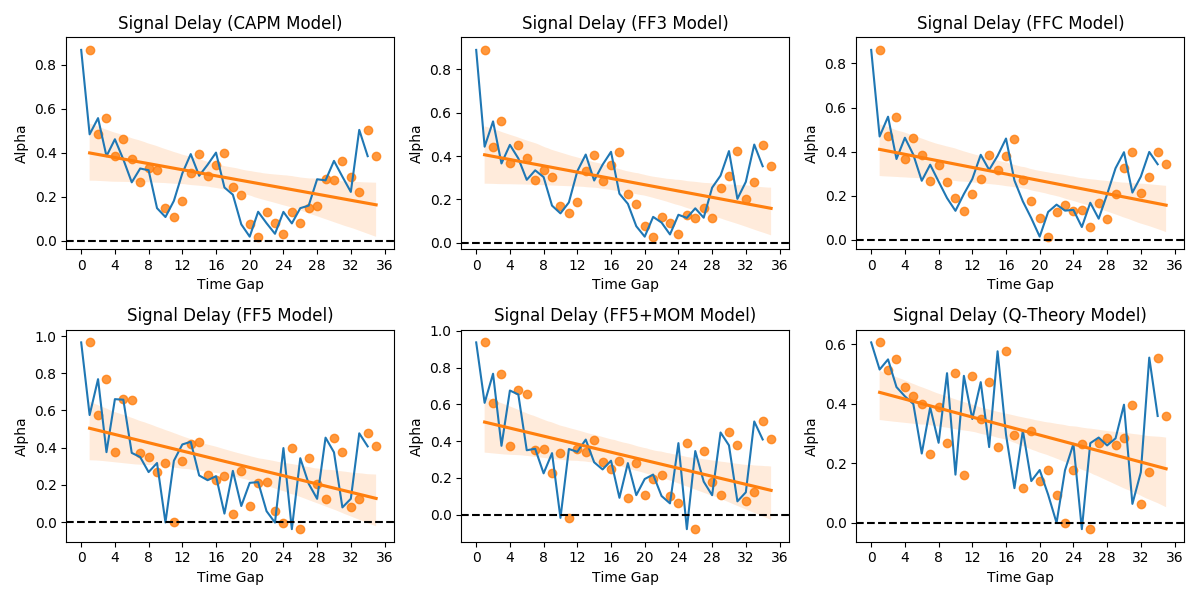
\includegraphics[width=\linewidth]{rfr_signal_delay.png}
    \caption{五组模型Q5-Q1结果(随机森林)}
    \label{signal1}
\end{figure}

\begin{figure}[htbp]
  \centering
    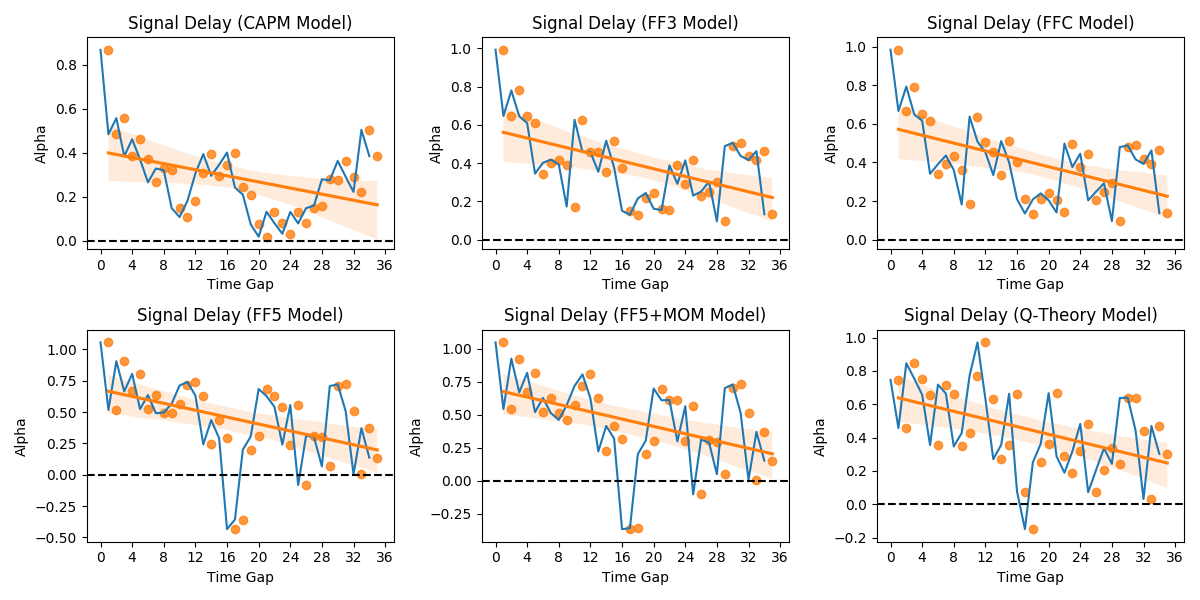
\includegraphics[width=\linewidth]{gbr_signal_delay.png}
    \caption{五组模型Q5-Q1结果(GBDT)}
    \label{signal2}
\end{figure}

在五组模型中,多空组合收益均在当前时点$t$拥有最高的超额收益$\alpha$,但后面随着时间增长,收益呈现明显的下降趋势,说明当前时点的错误定价已经随着时间而归正,股票的市场价格能够灵活随着信息进行调整,进而逐渐趋近于内在价值,收益也就越来越小,证明了本文在每一期重新进行内在价值计算、根据错误定价因子M对公司进行分组的正确性。若采用过往时点的结果进行未来股票收益的分析,会产生一定的偏误,所以要做到信息的更新换代。
\begin{figure}[htbp]
  \centering
   \begin{subfigure}[b]{0.48\textwidth}
     \centering
    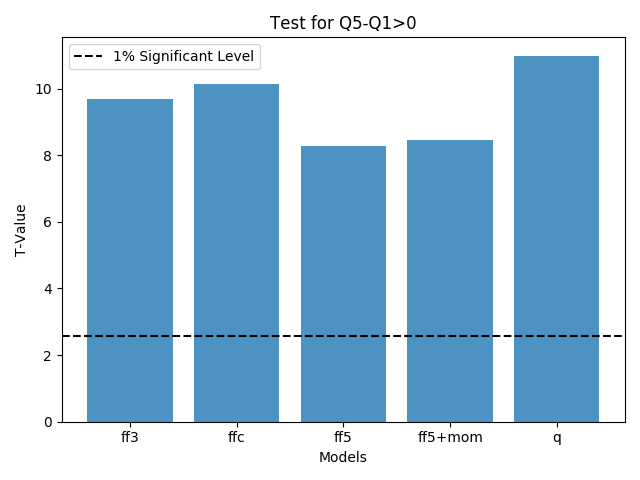
\includegraphics[width=\linewidth]{rfr_t_value.png}
    \caption{随机森林}
    \label{t1}
    \end{subfigure}
    \hfill
     \begin{subfigure}[b]{0.48\textwidth}
       \centering
    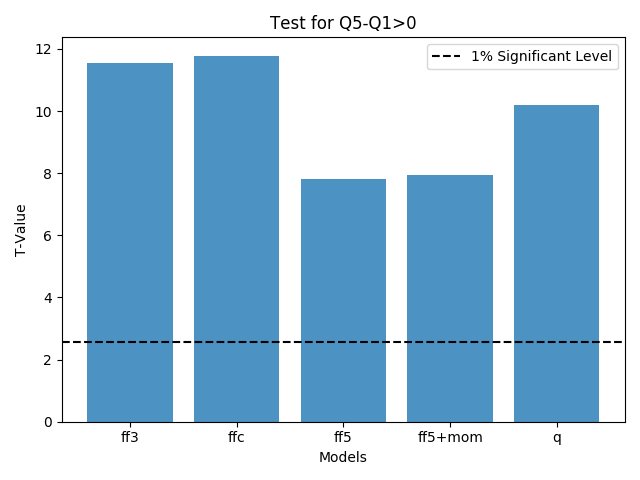
\includegraphics[width=\linewidth]{gbr_t_value.png}
    \caption{GBDT}
    \label{t2}
    \end{subfigure}
    \caption{五组模型多空组合显著性检验}
    \label{t}
\end{figure}

图~\ref{t}~是对于五组模型中多空组合收益是否显著大于0的检验,所有模型结果均在1\%的显著性水平下成立,证明了运用财务指标衡量公司内在价值的可行性、根据错误定价因子M进行公司分组的有效性。




%\subsection{原始代码}
%朴实的代码块:
%
%使用 verbatim 环境可以得到如下原样的输出。
%\begin{verbatim}
%print("Hello world!")
%\end{verbatim}
%
%使用 listings 包提供的 lstlisting 环境可以对代码进行进一步的格式化,minted 包所提供的 minted 环境还可以对代码进行高亮。更多定制功能请自行参照文档配置。
%
%\subsection{算法描述/伪代码}
%参考 \href{https://en.wikibooks.org/wiki/LaTeX/Algorithms}{Algorithms} 与 algorithm2e 文档,给出一个简单的示例,见算法 \ref{alg:alg1}。
%
%\begin{algorithm}
%  \SetAlgoLined
%  \KwData{this text}
%  \KwResult{how to write algorithm with \LaTeXe}
%  initialization\;
%  \While{not at end of this document}{
%    read current\;
%    \eIf{understand}{
%      go to next section\;
%      current section becomes this one\;
%    }{
%      go back to the beginning of current section\;
%    }
%  }
%  \caption{如何写算法}\label{alg:alg1}
%\end{algorithm}
%
%\section{绘图}
%关于使用 \LaTeX{} 绘图的更多例子,请参考 \href{https://www.overleaf.com/learn/latex/Pgfplots_package}{Pgfplots package}。一般建议使用如 Photoshop、PowerPoint 等制图,再转换成 PDF 等格式插入。
%
%\section{写在最后}
%工具不重要,对工具的合理运用才重要。希望本模板对大家的论文写作有所帮助。

% Chapter5

\chapter{实证分析}

\section{因子模型}\label{sfactor}
本文依据错误定价因子$M$的预测结果,构建了Q1和Q5两组的多空组合,以月度平均收益$mean$和风险调节收益$\alpha$作为绩效衡量指标。 为了避免A股市场做空机制的限制,本文还构建了Q1到Q5五组的多头组合,如果从Q1组到Q5组、从最被高估到最被低估的股票能够呈现超额收益的递增趋势,同样能证明错误定价因子$M$的有效性。

对于因子的选择,使用了常见的CAPM模型、Fama−French 三因子模型、 Carhart 四因子模型、Fama−French 五因子模型、以及Hou-Xue-Zhang 四因子模型(后称为q-因子模型),采用了其中的6组因子(CAPM、FF3、FFC、FF5、FF5+MOM、Q)进行研究,具体结果见表~\ref{factor}所示,记录了Q1到Q5五组多头组合和多空组合的月度平均收益$mean$、风险调节收益$\alpha$及$t$值。

\begin{table}[htbp]
\caption{因子模型回归}
\label{factor}
\begin{tabular*}{\hsize}{@{\hskip\tabcolsep\extracolsep\fill}*{8}{c}}
\toprule
模型                       & 系数                    & Q1 & Q2 & Q3 & Q4 & Q5 & Q5-Q1 \\ \midrule
 &$ mean$& -0.180&  0.037&0.255&0.421& 0.955&  1.135\\
 \multirow{2}{*}{CAPM}     & $\alpha$ &    0.0452         &    0.235&    0.540&    0.708&    1.153&   1.123\\
                         &$ t$值                     &     (0.52)         &   (2.71)         &   (6.24)         &   (7.80)         &   (8.26)  & (2.35)         \\
\multirow{2}{*}{FF3}     & $\alpha$ &      0.0793         &    0.271&    0.573&    0.747&    1.196&  1.096\\
                         & $t$值                     &    (0.93)         &   (3.18)         &   (6.72)         &   (8.39)         &   (8.65)      &(2.43)     \\
\multirow{2}{*}{FFC}     & $\alpha$  &  0.146  &    0.320&    0.643&    0.823&    1.268 & 1.099\\
                         &$ t$ 值                   &    (1.70)         &   (3.74)         &   (7.52)         &   (9.22)         &   (9.13)    &(2.40)       \\
\multirow{2}{*}{FF5}     &$\alpha$  & -1.186&   -1.172&   -0.941&   -0.762&   -0.143      & 0.981\\
                         & $t$  值                   &   (-9.02)         & (-12.90)         &  (-9.76)         &  (-9.01)         &  (-2.82)   &   (1.76)      \\
\multirow{2}{*}{FF5+mom} &$\alpha$  & -1.122&   -1.116&   -0.869&   -0.687&  -0.0727  &  0.984    \\
                         &$ t $ 值        &        (-11.14)         & (-11.12)         &  (-8.69)         &  (-6.56)         &  (-0.44)  & (1.75)  \\
\multirow{2}{*}{Q}       &$\alpha$  &   0.177&    0.380&    0.677&    0.853&    1.298    &1.106\\
                         & $t$   值                  &     (2.08)         &   (4.46)         &   (7.95)         &   (9.58)         &   (9.37)  &(2.43)     \\ \bottomrule
\end{tabular*}
\end{table}

可以看出在运用BRTs模型进行数据模拟后,Q1到Q5的多头组合月度平均收益$mean$、风险调节收益$\alpha$均呈现递增趋势,并且非常显著;Q1、Q5的多空组合也有显著的正收益,证明了错误定价因子$M$的作用,以及基本面分析的有效性。

附录~\ref{linear}~展现了采用线性回归方法的因子模型结果,可以看出结果也非常显著,佐证了本文的结论。
但相比而言,采用BRTs算法得到的Q1、Q5的多空组合收益率更高;
并且BRTs算法能够有效处理缺失值的问题,而线性回归对于缺失值非常敏感,数据量大大缩水,虽然两种方法结果相似,但对于结果或多或少仍有影响,如果扩展到其他研究中,这种数据的直接丢弃或许是致命的。

\section{Fama-MacBeth截面回归}\label{sfmb}
表~\ref{fmb}~展现了对于所有公司Fama-MacBeth的时间序列截面回归结果,两列分别选用了不同的控制变量来表现错误定价因子M的预测能力,所有列均控制了行业固定效应,括号内的数字代表$t$值。

其中,第一列仅采用了$M$作为解释变量,结果非常显著;第二列新加入了公司特征作为控制变量:$beta$值、市净率$BM$、三个动量因子$lagretn$、$mom12$、$mom36$、市盈率$EP$、净经营性资产增长率$grltnoa$与毛利率$PA$,让回归更为完整,错误定价因子$M$同样显著,说明错误定价因子$M$可以用来预测股票未来收益。

\begin{table}[htbp]\centering
\def\sym#1{\ifmmode^{#1}\else\(^{#1}\)\fi}
\caption{Fama-MacBeth截面回归}
\label{fmb}
\begin{tabular*}{0.85\hsize}{@{\hskip\tabcolsep\extracolsep\fill}*{3}{c}}
\toprule
        &\multicolumn{1}{c}{(1)}&\multicolumn{1}{c}{(2)}\\
 &\multicolumn{1}{c}{$R_{t+1}$}&\multicolumn{1}{c}{$R_{t+1}$}\\
\midrule
$M$         &    1.623\sym{***}&    6.601\sym{**} \\
          &  (10.82)         &   (1.98)         \\
$beta  $    &                  &    20.08\sym{***}\\
          &                  &   (8.23)         \\
$BM  $      &                  &    27.61         \\
          &                  &   (1.48)         \\
$EP  $      &                  &   -252.2         \\
          &                  &  (-0.52)         \\
$lagretn $  &                  &   -13.03\sym{***}\\
          &                  &  (-3.39)         \\
$mom12  $   &                  &    8.121\sym{***}\\
          &                  &   (5.43)         \\
$mom36  $   &                  &    3.545\sym{**} \\
          &                  &   (2.42)         \\
$grltnoa $  &                  &   -0.757         \\
          &                  &  (-0.17)         \\
$PA   $     &                  &   -176.7\sym{*}  \\
          &                  &  (-1.80)         \\
行业固定效应&    控制   &    控制   \\
\midrule
$N$         &   129169         &    50153     \\
$R^2$        &   0.0557         &    0.572     \\
\bottomrule
\multicolumn{3}{l}{\footnotesize \textit{t} statistics in parentheses}\\
\multicolumn{3}{l}{\footnotesize \sym{*} \(p<0.1\), \sym{**} \(p<0.05\), \sym{***} \(p<0.01\)}\\
\end{tabular*}
\end{table}

\section{股票特征重要性}
如图~\ref{feature}~所示,在对公司内在价值的回归计算过程中,对51个财务指标进行重要性排序。其中,$y$轴显示了所有财务指标,$x$轴代表了不同财务指标的重要性比例,可见最为重要的指标有股本、净利润,分别占到了约10\%、6\%,对应说明评估公司内在价值的重要因素一般在于股东行为以及公司业务的利润大小等。

\begin{figure}[htbp]
  \centering
    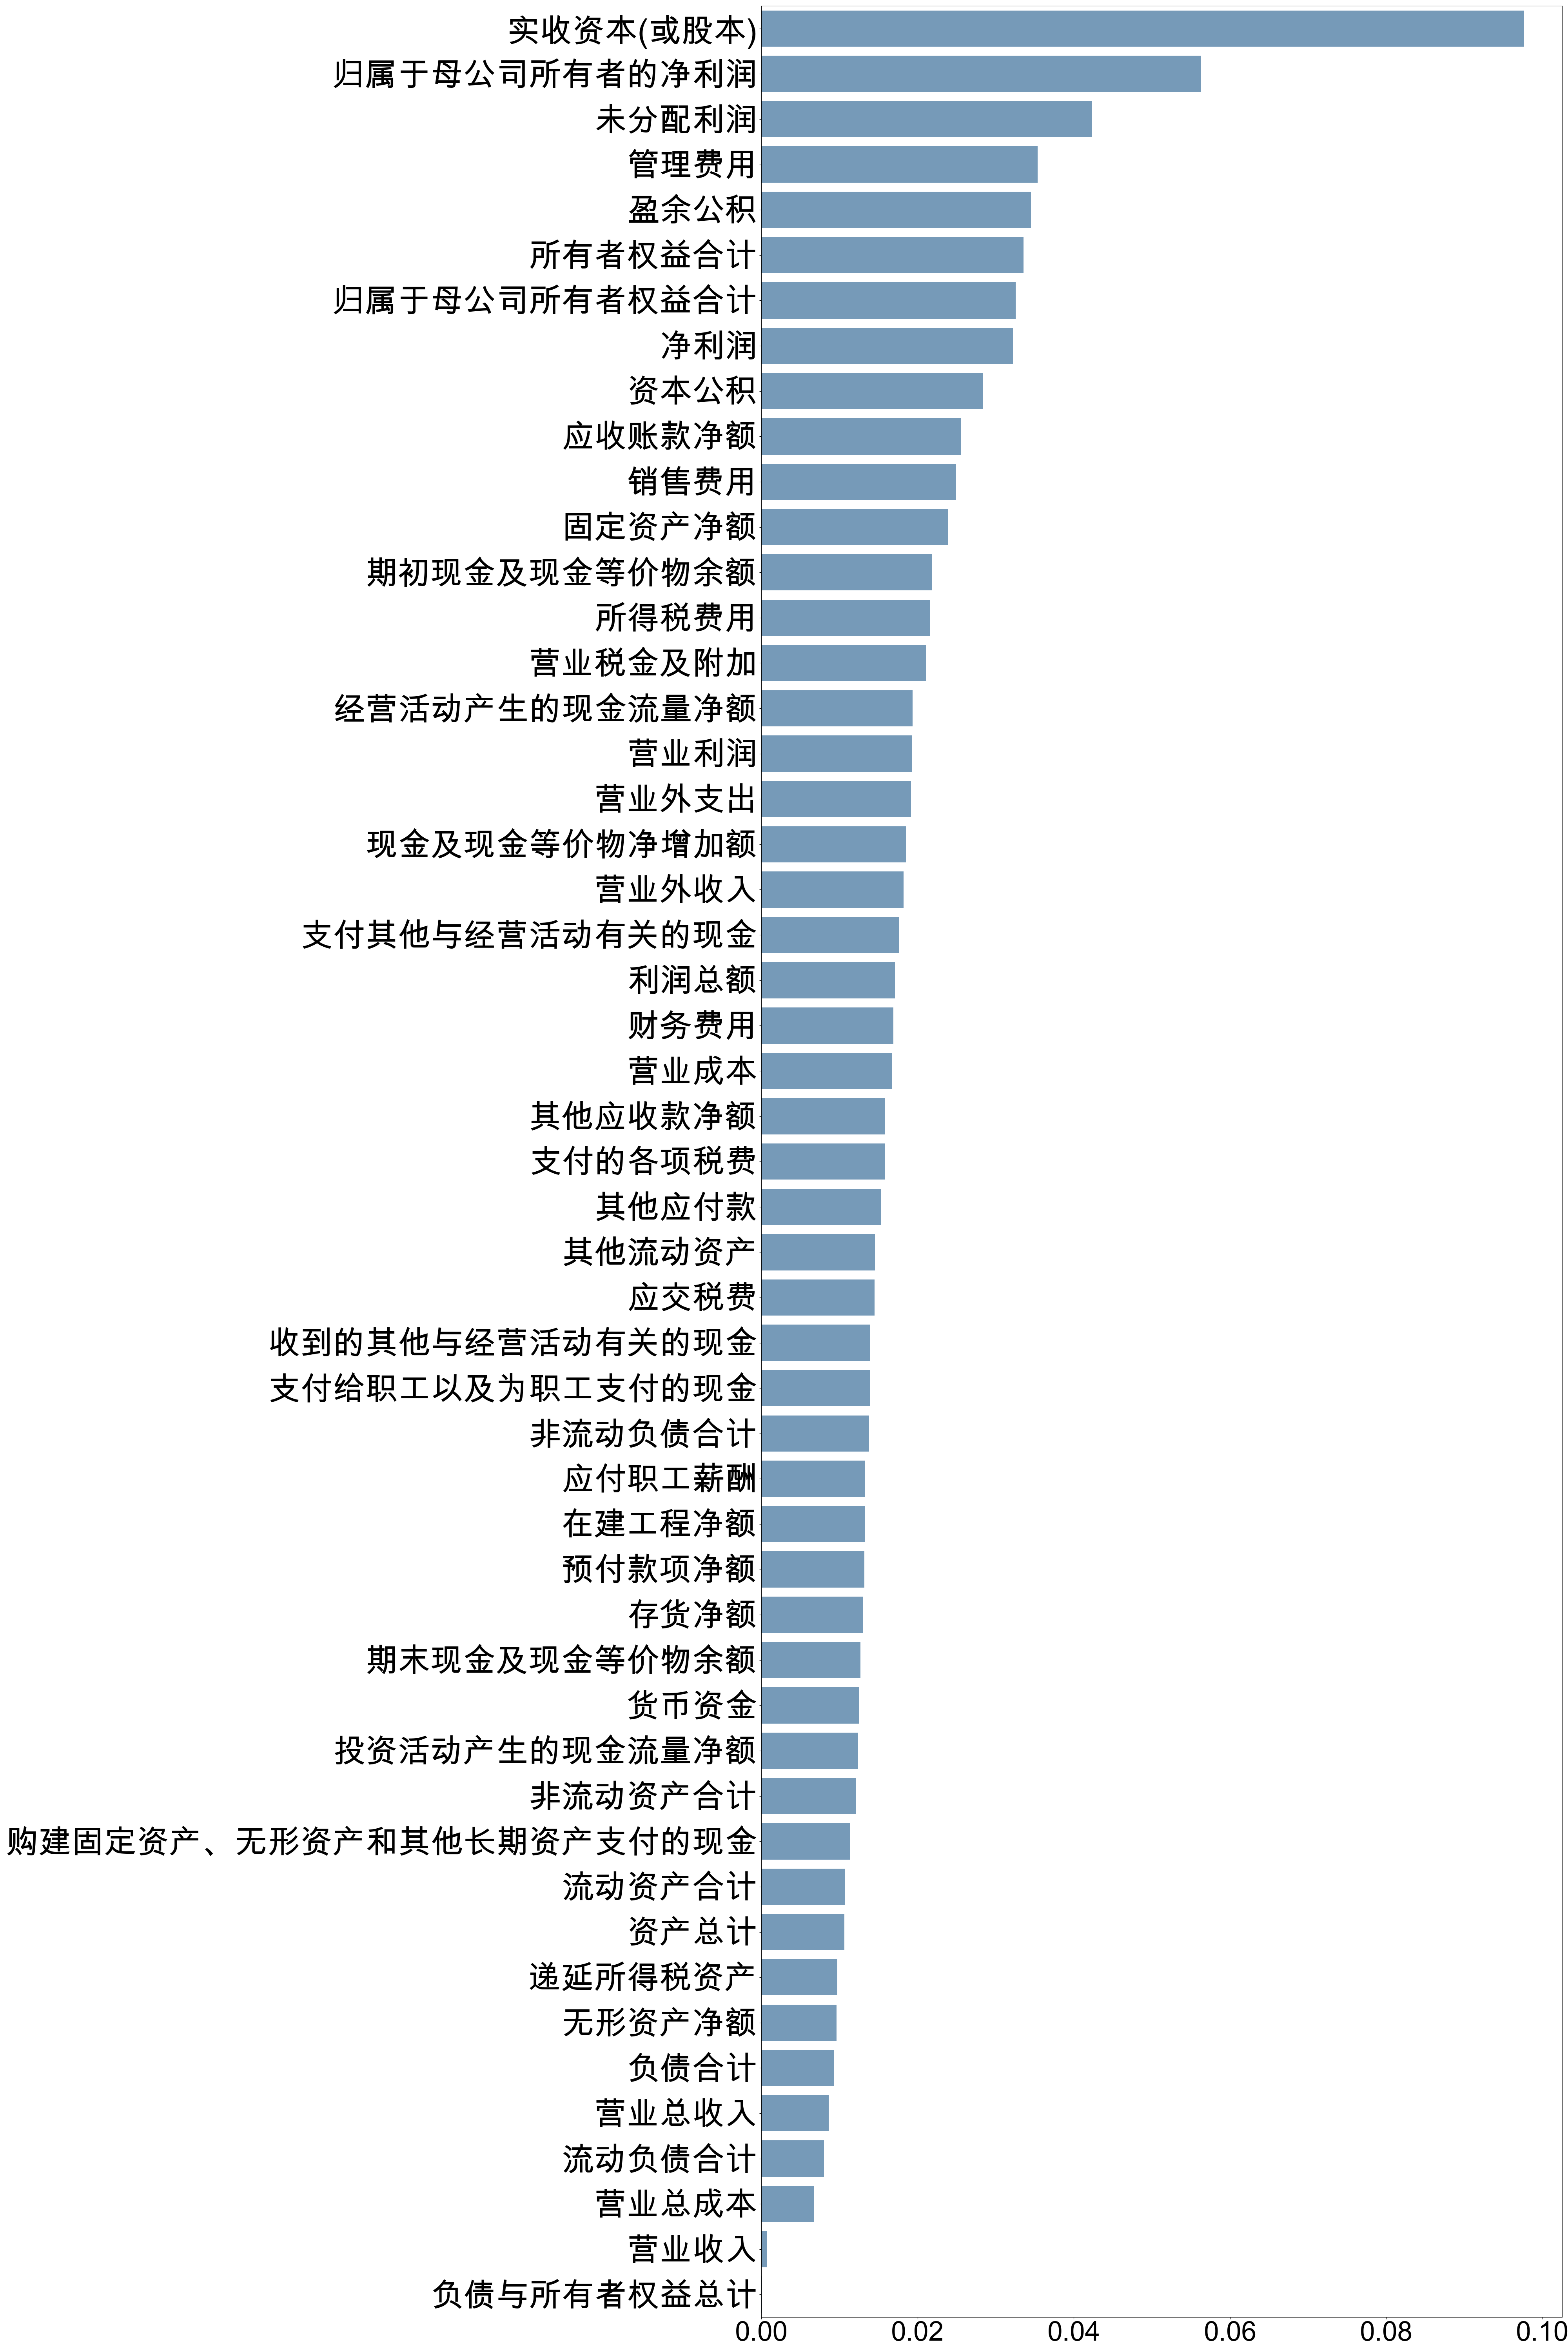
\includegraphics[width=\linewidth]{feature importance1.png}
    \caption{股票特征重要性}
    \label{feature}
\end{figure}

\section{稳健性分析}
上述小节~\ref{sfmb}、\ref{sfactor}~的结果证明了错误定价因子$M$以及基本面分析的有效性,公司内在价值能够完全反映于财务指标。为检验超额利润是否真正来自于错误定价而非因子遗漏,即市场价值是否会逐渐趋向于内在价值,本文进行以下稳健性分析。

在第$t$期计算各公司的错误定价因子$M$,并分为Q1到Q5五组,构建Q1与Q5两组的多空组合,基于该投资组合计算未来36期的收益情况,同上文采用六组因子(CAPM、FF3、FFC、FF5、FF5+MOM、Q)进行研究,结果如图~\ref{signal1}、\ref{signal2}、\ref{signal3}、\ref{signal4}、\ref{signal5}、\ref{signal6}~所示。

\begin{figure}[htbp]
  \centering
    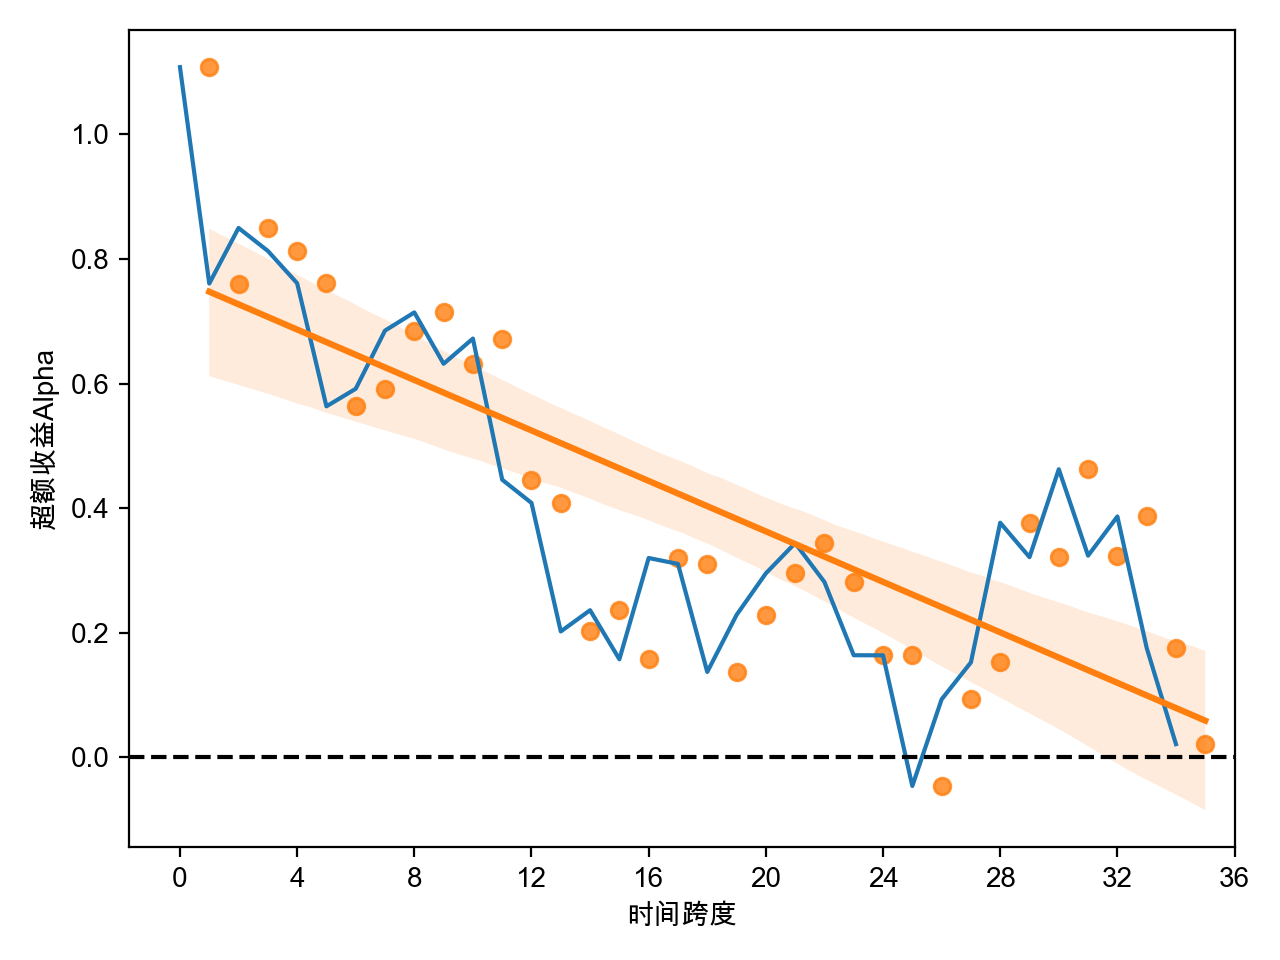
\includegraphics[width=\linewidth]{signal delay1.png}
    \caption{信号延迟(CAPM模型)}
    \label{signal1}
\end{figure}
     
\begin{figure}[htbp]
  \centering
    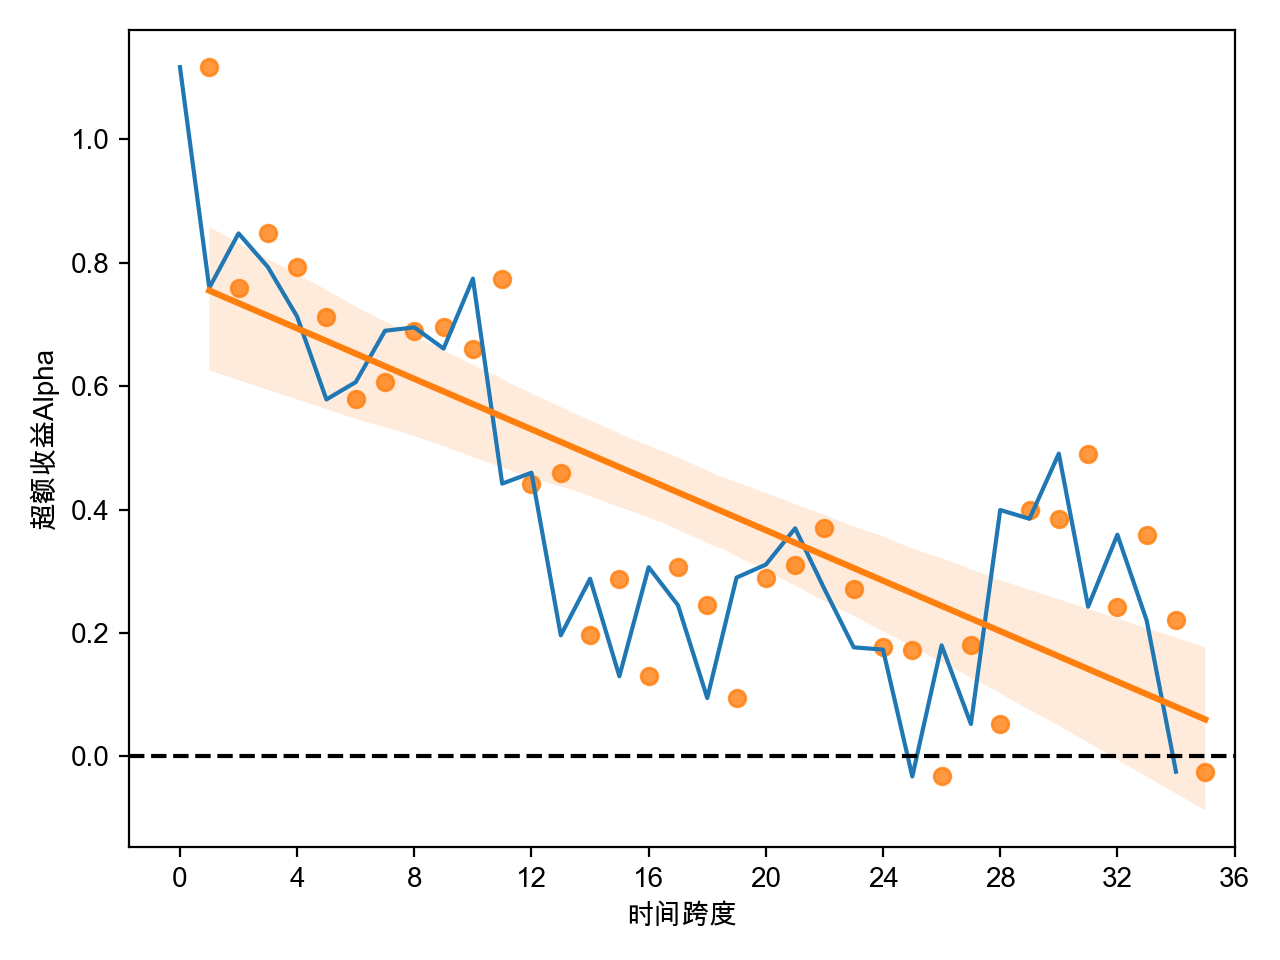
\includegraphics[width=\linewidth]{signal delay2.png}
    \caption{信号延迟(FF3模型)}
    \label{signal2}
\end{figure}

\begin{figure}[htbp]
  \centering
    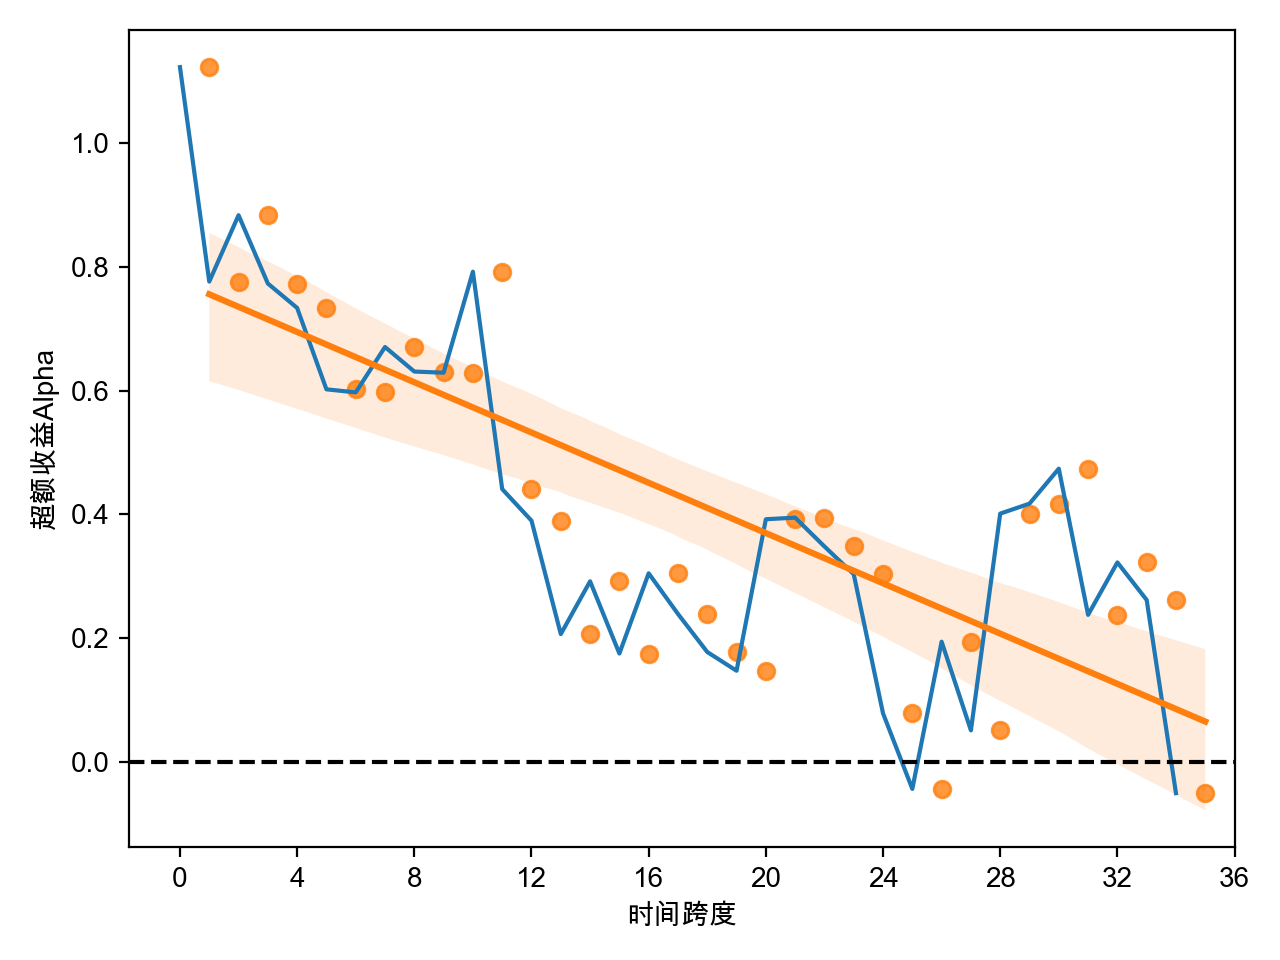
\includegraphics[width=\linewidth]{signal delay3.png}
    \caption{信号延迟(FFC模型)}
    \label{signal3}
\end{figure}
  
\begin{figure}[htbp]
  \centering
    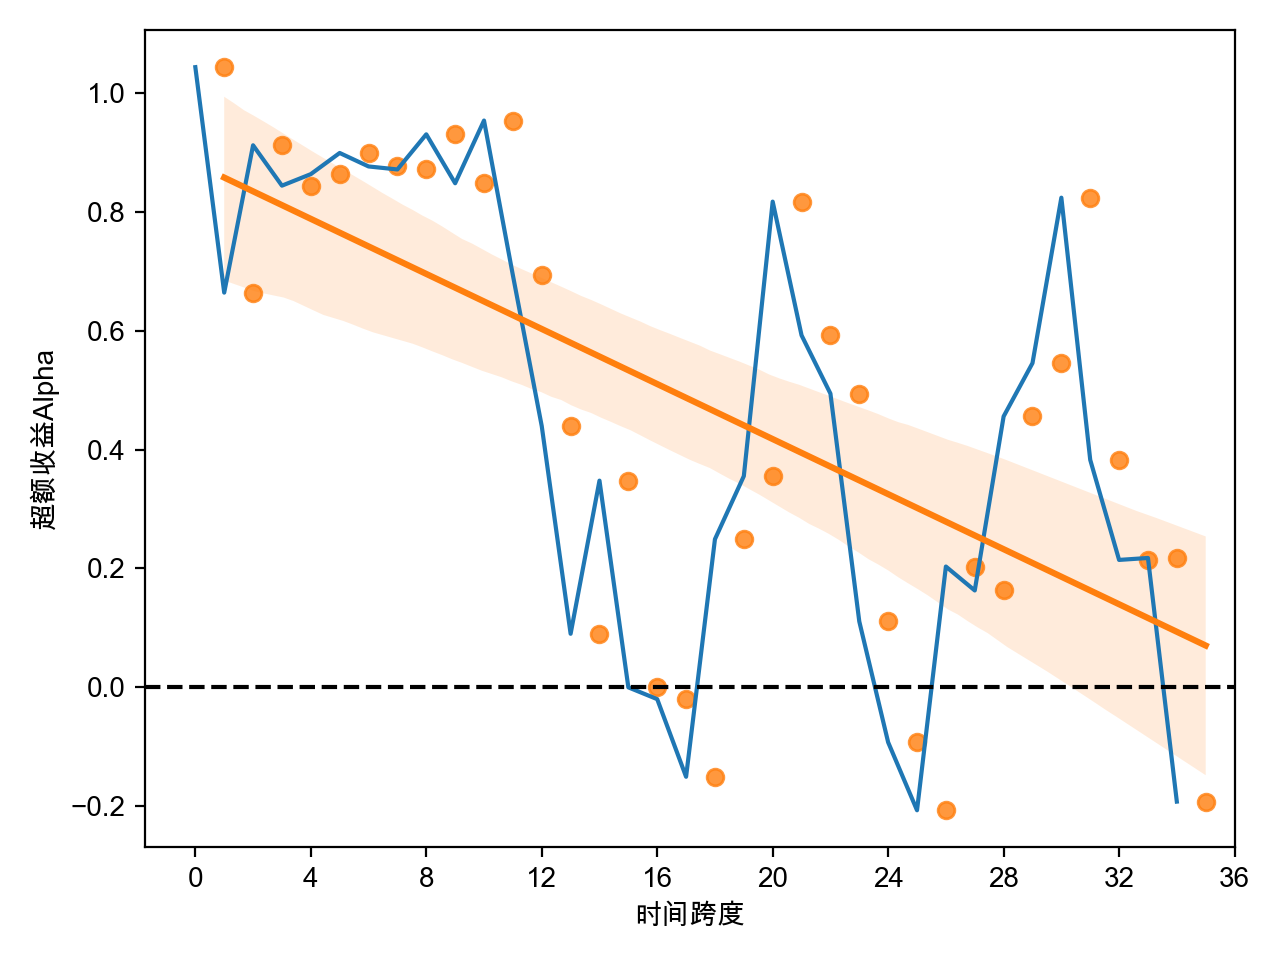
\includegraphics[width=\linewidth]{signal delay4.png}
    \caption{信号延迟(FF5模型)}
    \label{signal4}
\end{figure}

\begin{figure}[htbp]
  \centering
    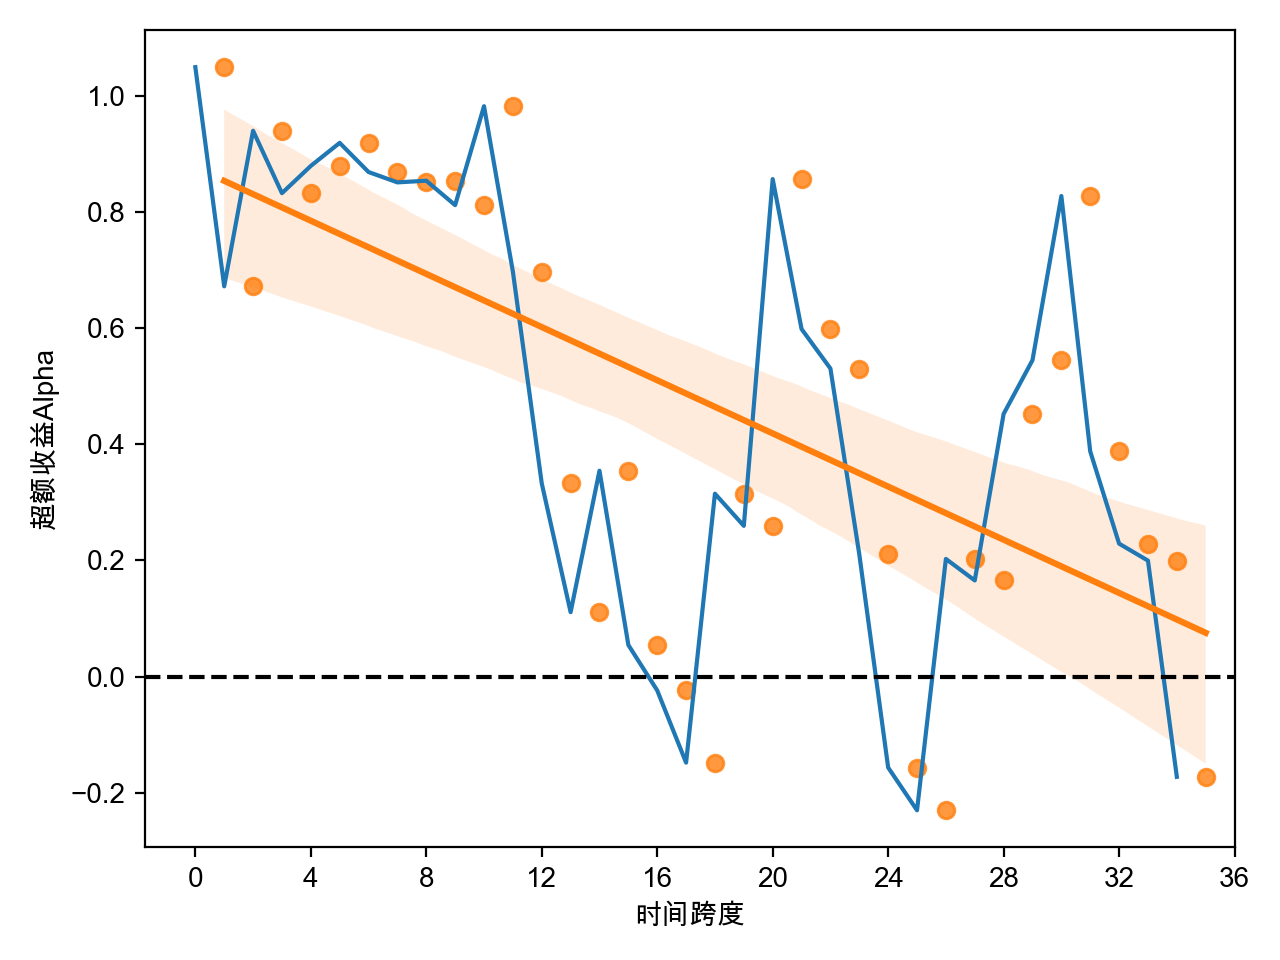
\includegraphics[width=\linewidth]{signal delay5.png}
    \caption{信号延迟(FF5+MOM模型)}
    \label{signal5}
\end{figure}
  
\begin{figure}[htbp]
  \centering
    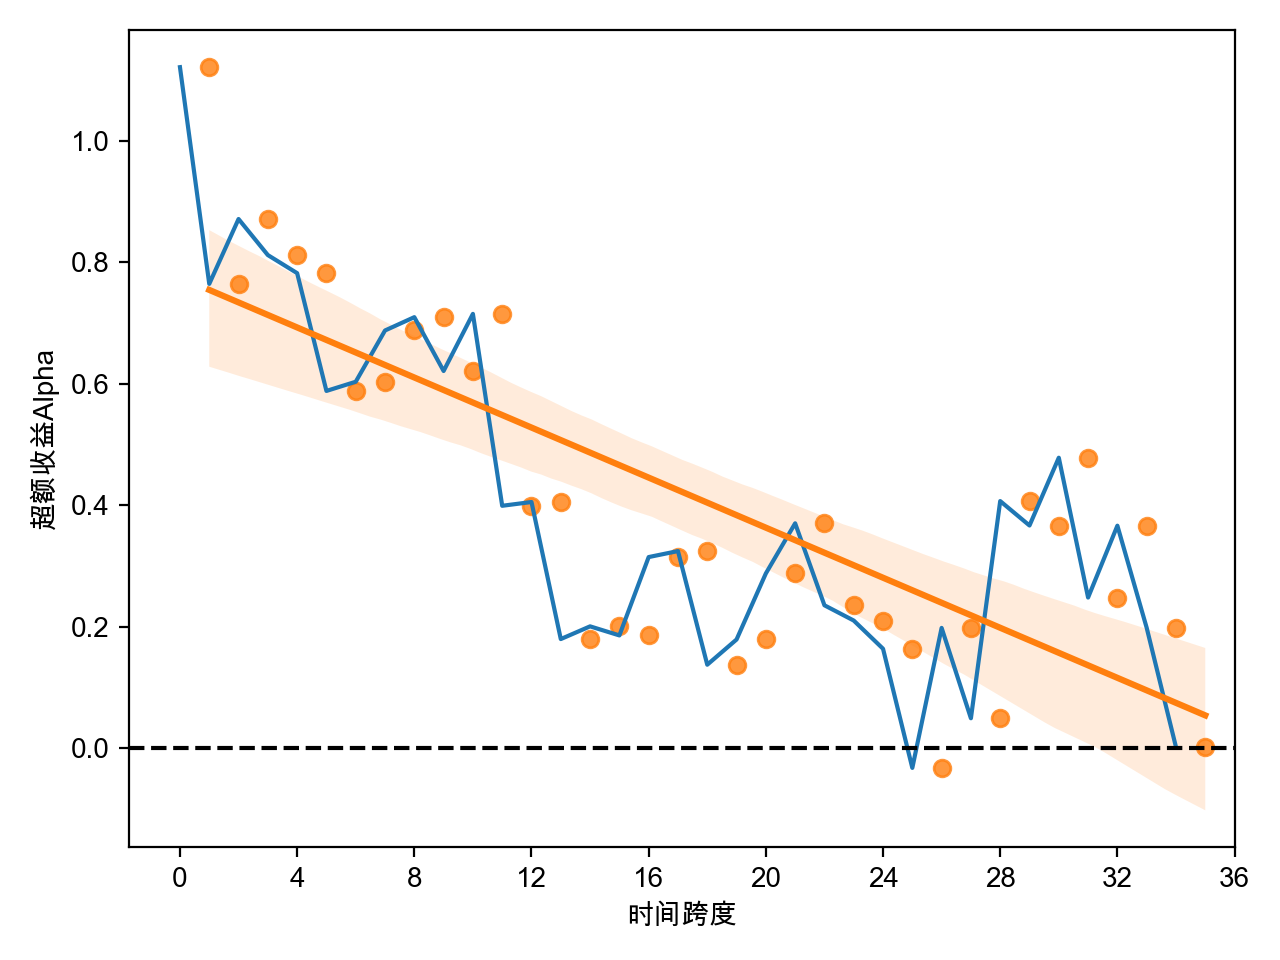
\includegraphics[width=\linewidth]{signal delay6.png}
    \caption{信号延迟(Q因子模型)}
    \label{signal6}
\end{figure}

在六组模型中,多空组合收益均在当前第$t$期拥有最高的超额收益$\alpha$,但后面随着时间增长,收益呈现明显的下降趋势,说明当前时点的错误定价已经随着时间而抵消,股票的市场价格能够灵活随着信息进行调整,进而逐渐趋近于内在价值,收益也就越来越小,证明了本文在每一期重新进行内在价值计算、根据错误定价因子$M$对公司进行分组的正确性。若采用过往时点的结果进行未来股票收益的分析,会产生一定的偏误,所以对于运用错误定价因子$M$进行投资组合的构建,要做到及时更新。

\begin{figure}[htbp]
  \centering
    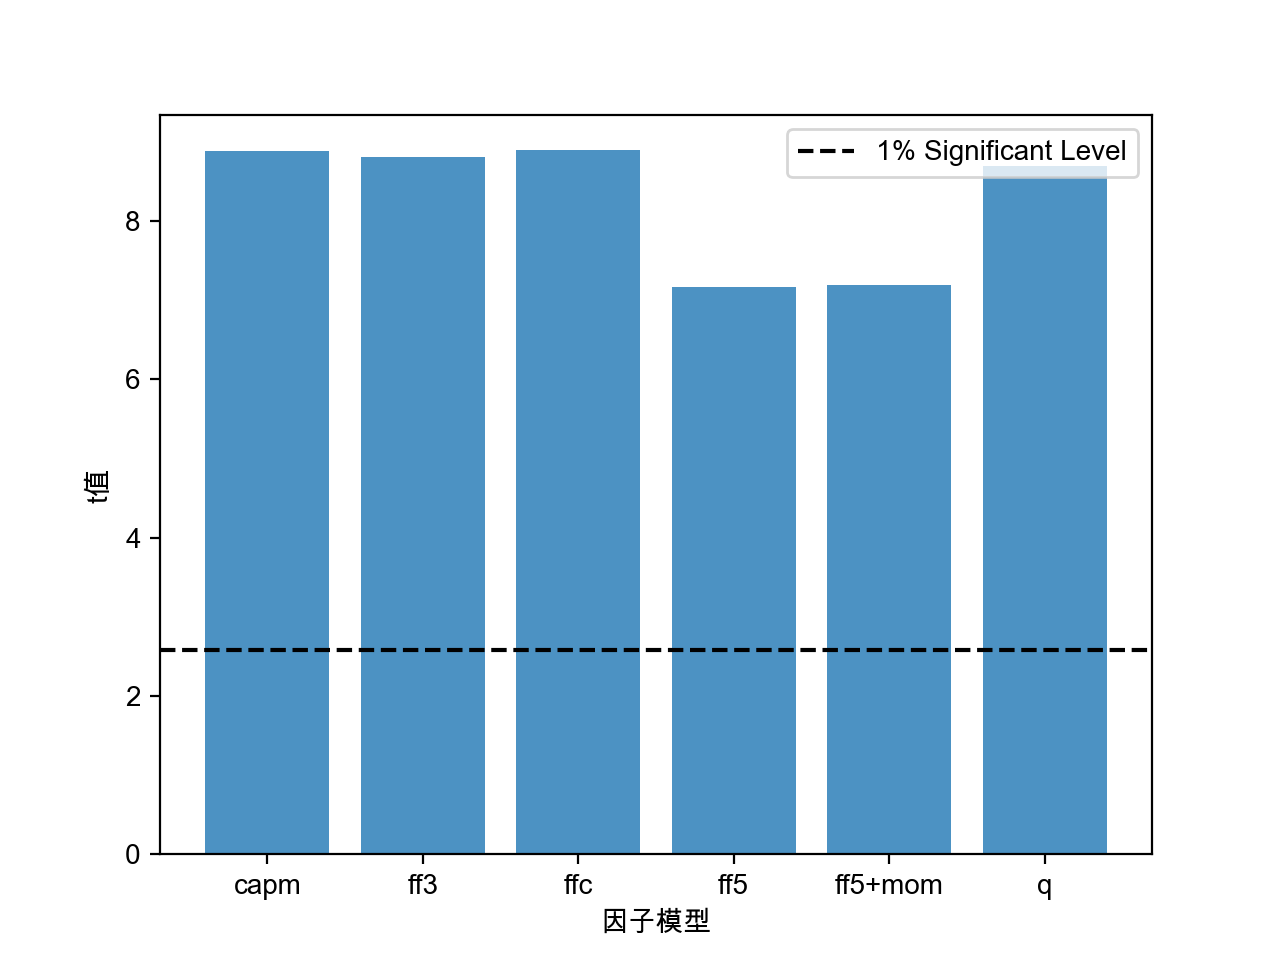
\includegraphics[width=\linewidth]{t_value.png}
      \caption{五组模型多空组合显著性检验}
    \label{t}
\end{figure}

图~\ref{t}~是对于六组因子模型中多空组合收益是否显著大于0的检验,所有模型结果均在1\%的显著性水平下成立,证明了运用财务指标衡量公司内在价值的可行性、根据错误定价因子$M$进行公司分组的有效性。



\end{document}